%\VignetteEngine{knitr::knitr}
% some terminal commands to copy once and scroll when needed
% cd '/mnt/Hitachi2GB/00NMML/activePapers/KrigLinCaution/KrigLinCaution_package/KrigLinCaution/inst/doc'
% cd '/home/jay/Data/KrigLinCaution/KrigLinCaution_package/KrigLinCaution/inst/doc'
% Rscript -e "library(knitr); knit('KrigLinCaution.Rnw')"
% Rscript -e "library(knitr); purl('KrigLinCaution.Rnw')"
% pdflatex KrigLinCaution
% bibtex KrigLinCaution

\documentclass[11pt, titlepage]{article}\usepackage[]{graphicx}\usepackage[]{color}
%% maxwidth is the original width if it is less than linewidth
%% otherwise use linewidth (to make sure the graphics do not exceed the margin)
\makeatletter
\def\maxwidth{ %
  \ifdim\Gin@nat@width>\linewidth
    \linewidth
  \else
    \Gin@nat@width
  \fi
}
\makeatother

\definecolor{fgcolor}{rgb}{0.345, 0.345, 0.345}
\newcommand{\hlnum}[1]{\textcolor[rgb]{0.686,0.059,0.569}{#1}}%
\newcommand{\hlstr}[1]{\textcolor[rgb]{0.192,0.494,0.8}{#1}}%
\newcommand{\hlcom}[1]{\textcolor[rgb]{0.678,0.584,0.686}{\textit{#1}}}%
\newcommand{\hlopt}[1]{\textcolor[rgb]{0,0,0}{#1}}%
\newcommand{\hlstd}[1]{\textcolor[rgb]{0.345,0.345,0.345}{#1}}%
\newcommand{\hlkwa}[1]{\textcolor[rgb]{0.161,0.373,0.58}{\textbf{#1}}}%
\newcommand{\hlkwb}[1]{\textcolor[rgb]{0.69,0.353,0.396}{#1}}%
\newcommand{\hlkwc}[1]{\textcolor[rgb]{0.333,0.667,0.333}{#1}}%
\newcommand{\hlkwd}[1]{\textcolor[rgb]{0.737,0.353,0.396}{\textbf{#1}}}%
\let\hlipl\hlkwb

\usepackage{framed}
\makeatletter
\newenvironment{kframe}{%
 \def\at@end@of@kframe{}%
 \ifinner\ifhmode%
  \def\at@end@of@kframe{\end{minipage}}%
  \begin{minipage}{\columnwidth}%
 \fi\fi%
 \def\FrameCommand##1{\hskip\@totalleftmargin \hskip-\fboxsep
 \colorbox{shadecolor}{##1}\hskip-\fboxsep
     % There is no \\@totalrightmargin, so:
     \hskip-\linewidth \hskip-\@totalleftmargin \hskip\columnwidth}%
 \MakeFramed {\advance\hsize-\width
   \@totalleftmargin\z@ \linewidth\hsize
   \@setminipage}}%
 {\par\unskip\endMakeFramed%
 \at@end@of@kframe}
\makeatother

\definecolor{shadecolor}{rgb}{.97, .97, .97}
\definecolor{messagecolor}{rgb}{0, 0, 0}
\definecolor{warningcolor}{rgb}{1, 0, 1}
\definecolor{errorcolor}{rgb}{1, 0, 0}
\newenvironment{knitrout}{}{} % an empty environment to be redefined in TeX

\usepackage{alltt}
\usepackage{geometry}
\geometry{verbose,letterpaper,tmargin=2.54cm,bmargin=2.54cm,lmargin=2.54cm,rmargin=2.54cm}
\usepackage{graphicx, ams, amsmath, amssymb, natbib, setspace, bm}
\usepackage{float}
\usepackage{multirow}
\usepackage{mathrsfs}
\usepackage{relsize}
\usepackage{subcaption}
\usepackage{pdflscape}
\usepackage{pgf}
\usepackage{arydshln}
\usepackage{/mnt/Hitachi2GB/shTex/mymacros}
%\usepackage{/home/jay/Data/shTex/mymacros}
\usepackage{bbding}
\usepackage{lineno}
\usepackage{fancyvrb}
\usepackage[shortlabels]{enumitem}
\linenumbers
\setlength{\parindent}{3em}
%\onehalfspacing
\doublespacing
\usepackage{lipsum}
\usepackage{setspace}
\usepackage{etoolbox}
\AtBeginEnvironment{tabular}{\singlespacing}
\pdfpagewidth 8.5in
\pdfpageheight 11in
\setlength{\oddsidemargin}{0.0in} \setlength{\textwidth}{6.5in}
\setlength{\topmargin}{0.15in} \setlength{\textheight}{8.5in}
\setlength{\headheight}{0.0in} \setlength{\headsep}{0.0in}
%\renewcommand{\abstractname}{Summary}
%\renewcommand{\theequation}{(\arabic{equation})}
\setcounter{figure}{0}
\makeatletter
\renewcommand{\theequation}{eqn \arabic{equation}}
\renewcommand\tagform@[1]{\maketag@@@{\ignorespaces#1\unskip\@@italiccorr}}
\setlength{\tabcolsep}{5pt}     
\renewcommand{\arraystretch}{1}
\makeatother
\newcommand{\argminE}{\mathop{\mathrm{argmin}}}
\IfFileExists{upquote.sty}{\usepackage{upquote}}{}
\begin{document}


% ------------------------------------------------------------------------------
% ------------------------------------------------------------------------------
% 																	TITLE
% ------------------------------------------------------------------------------
% ------------------------------------------------------------------------------

\titlepage
\title {Kriging Models for Linear Networks and non-Euclidean Distances: Cautions and Solutions}
\author{Jay M. Ver Hoef \\
\hrulefill \\ 
Marine Mammal Laboratory, NOAA Fisheries Alaska Fisheries Science Center\\
7600 Sand Point Way NE, Seattle, WA 98115\\
tel: (907) 347-5552 \hspace{.5cm} E-mail: jay.verhoef@noaa.gov\\
\hrulefill \\
}

\maketitle

% ------------------------------------------------------------------------------
% ------------------------------------------------------------------------------
% ------------------------------------------------------------------------------
% 														   	ABSTRACT
% ------------------------------------------------------------------------------
% ------------------------------------------------------------------------------
% ------------------------------------------------------------------------------
\renewcommand{\abstractname}{Summary}
\begin{abstract}
\begin{onehalfspace}

\begin{enumerate}
  \item There are now many examples where ecological researchers used non-Euclidean distance metrics in geostatistical models that were designed for Euclidean distance, such as those used for kriging.  This can lead to problems where predictions have negative variance estimates.  Technically, this occurs because the spatial covariance matrix, which depends on the geostatistical models, is not guaranteed to be positive definite when non-Euclidean distance metrics are used.  These are not permissible models, and should be avoided.
  \item I give a quick review of kriging and illustrate the problem with several simulated examples, including locations on a circle, locations on a linear dichotomous network (such as might be used for streams), and locations on a linear trail or road network. I re-examine the linear-network distance models from \citet{Ladl:Avga:Whea:Boyc:pred:2016} and show that they are not guaranteed to have a positive-definite covariance matrix.
  \item  I introduce the reduced-rank method, also called a predictive-process model, for creating valid spatial covariance matrices with non-Euclidean distance metrics.  It has an additional advantage of fast computation for large data sets.
  \item I reanalyzed the data of \citet{Ladl:Avga:Whea:Boyc:pred:2016}, showing that fitted models that used linear network distance in geostatistical models, both with and without a nugget effect, had negative variances, poor predictive performance compared reduced-rank methods, and had improper coverage for the prediction intervals. The reduced-rank approach using linear network distances provided a class of permissible models that had better predictive performance and proper coverage for the prediction intervals, and could be combined with Euclidean distance models to provide the best overall predictive performance. 
\end{enumerate}
\end{onehalfspace}
\hrulefill \\

\noindent {\sc Key Words:} spatial statistics, geostatistics, prediction, reduced-rank methods, predictive process models\\

\end{abstract}

% ------------------------------------------------------------------------------
% ------------------------------------------------------------------------------
% ------------------------------------------------------------------------------
% 															INTRODUCTION
% ------------------------------------------------------------------------------
% ------------------------------------------------------------------------------
% ------------------------------------------------------------------------------

\newpage
\begin{spacing}{1.9}
\begin{flushleft}
\setlength{\parindent}{1cm}



\section*{INTRODUCTION}

There are now several examples in the ecological literature where, for spatial prediction like kriging, non-Euclidean distances were used in autocorrelation models developed under a Euclidean distance assumption.  This leads to a problem where prediction variances may be negative, and generally leads to unreliable standard errors for prediction.  My objective is to help ecologists understand the problem and avoid this mistake.  I introduce a class of models that are very easy to construct, based on linear mixed models, that perform well and guarantee that prediction standard errors will be positive.

\subsection*{A Quick Review of Kriging}

Kriging is a method for spatial interpolation, beginning as a discipline of atmospheric sciences in Russia, of geostatistics in France, and appearing in English in the early 1960's \citep{Gand:obje:1963, Math:Prin:1963,Cres:orig:1990}.  Kriging is attractive because it produces both predictions and prediction standard errors, providing uncertainty estimates for the predictions. Predictions and their standard errors are obtained after first estimating parameters of the kriging model.  The ordinary kriging model, which we will feature here, is,
\begin{equation} \label{eq:OKmodel}
    Y_i = \mu + Z_i + \varepsilon_i,
\end{equation}
where $Y_i$ is a spatial random variable at location $i$, $i = 1,2,\ldots,n$, with constant mean $\mu$ (the fixed effect), a zero-mean spatially autocorrelated error $Z_i$, and independent random error $ \varepsilon_i$. For the set $\{Z_i; i = 1,\ldots,n\}$, the spatial distance among locations is used to model autocorrelation among the random errors. Spatial autocorrelation is the tendency for spatial variables to co-vary, either in a similar fashion, or opposite from each other.  The most commonly observed type of spatial autocorrelation manifests as higher positive correlation among variables at sites closer together than among those at sites farther apart.  These tendencies are captured in autocorrelation and covariance matrices. 

Let $\bR$ be an autocorrelation matrix among spatial locations.  All of the diagonal elements of $\bR$ are ones. The off-diagonal element in the $i$th row and $j$th column of $\bR$ is the correlation, which lies between -1 and 1, between variables at site $i$ and site $j$.  Then a covariance matrix $\bC = \sigma^2_p\bR$ is just a scaled autocorrelation matrix that includes an overall variance, $\sigma^2_p$.  In constructing kriging models, practitioners often include a ``nugget'' effect, which is an independent (uncorrelated) random effect, $\varepsilon_i$, in \ref{eq:OKmodel} with variance $\sigma_0^2$.  The nugget effect is often ascribed to measurement error, or microscale variation, at a scale finer than the closest measurements in the data set.  Constructing a full covariance matrix for a kriging model generally yields
\begin{equation} \label{eq:bSigma}
	\bSigma = \bC + \sigma^2_0\bI = \sigma^2_p\bR + \sigma^2_0\bI,
\end{equation}
where $\sigma^2_p \ge 0$ is called the partial sill, $\sigma^2_0 \ge 0$ is the nugget effect, and $\bI$ is the identity matrix (a diagonal matrix of all ones). The total variance is $\sigma^2_p + \sigma^2_0$.  The off-diagonal elements of $\bR$ are obtained from models that generally decrease as distance increases, with a few that also oscillate. Several autocorrelation models \citep[][p. 80--93]{Chil:Delf:geos:1999}, based on Euclidean distance, $d_{i,j}$, between sites $i$ and $j$, are
\begin{equation} \label{eq:autocorrModels}
	\begin{array}{l}
  \rho_{e}(d_{i,j}) = \exp(-d_{i,j}/\alpha), \\
  \rho_{s}(d_{i,j}) = [1 - 1.5(d_{i,j}/\alpha) + 0.5(d_{i,j}/\alpha)^3] \cI(d_{i,j} < \alpha), \\
  \rho_{g}(d_{i,j}) = \exp(-(d_{i,j}/\alpha)^2), \\
	\rho_{c}(d_{i,j}) = 1/(1+(d_{i,j}/\alpha)^2), \\
	\rho_{h}(d_{i,j}) = (\alpha/d_{i,j})\sin(d_{i,j}/\alpha)\cI(d_{i,j} > 0) + \cI(d_{i,j} = 0),
	\end{array}
\end{equation}
where distances are scaled by $\alpha \ge 0$, called the range parameter. $\cI(a)$ is an indicator function, equal to one if the argument $a$ is true, otherwise it is zero.

Examples of the autocorrelation models in \ref{eq:autocorrModels}, scaled with a partial sill, $\sigma^2_p = 2$, and a nugget effect, $\sigma^2_0 = 1$, are shown in Figure~\ref{fig:autocorrModels}a.  The exponential model, $\rho_e(d_{i,j})$, is commonly used, and a special case of the Matern model that approaches zero autocorrelation asymptotically (Figure~\ref{fig:autocorrModels}c). The spherical model, $\rho_s(d_{i,j})$, also is common, attaining exactly zero autocorrelation at $\alpha$ (Figure~\ref{fig:autocorrModels}d).  Both the exponential and spherical models decrease rapidly near the origin, for short distances, whereas the Gaussian model, $\rho_g(d_{i,j})$, decreases more slowly near the origin. The Gaussian model occurs as a limiting case for the smoothness parameter of the Matern model, and creates very smooth spatial surfaces. The Cauchy model, $\rho_c(d_{i,j})$ is similar to the Gaussian, but approaches zero autocorrelation very slowly. Finally, The hole effect model, $\rho_h(d_{i,j})$ allows for negative autocorrelation in a dampened oscillating manner. These models highlight different features of autocorrelation models, and they will be used throughout this paper. Many more models are given in \citet[][p. 80--93]{Chil:Delf:geos:1999}.  Autocorrelation is generally controlled by $\alpha$, which must estimated from real data.  However, it is useful to vary $\alpha$ through simulated data, and even for real distance data, to understand its effect on covariance models, which I do in Figures~1c,d, and also in Figures 2 and 3.

Kriging is often expressed as semivariograms rather than autocorrelation models.  Semivariograms model the variance of the \emph{difference} among variables. If $Y_i$ and $Y_j$ are random variables at spatial locations $i$ and $j$, respectively, a semivariogram is defined as $\gamma(d_{i,j}) \equiv \textrm{E}(Y_i - Y_j)^2/2$, where E is expectation.  All of the models in \ref{eq:autocorrModels} can be written as semivariograms,
\begin{equation} \label{eq:semivarrho}
				\gamma_m(d_{i,j}) = \sigma^2_p(1 - \rho_m(d_{i,j})),
\end{equation}
where $m = e, s, g, c,$ or $h$ for exponential, spherical, Gaussian, Cauchy, or hole effect, respectively. Figure~\ref{fig:autocorrModels}b shows semivariograms that are equivalent to the models in Figure~\ref{fig:autocorrModels}a.  A matrix of semivariogram values among spatial locations can be written in terms of \ref{eq:bSigma},
\[
\bGamma = (\sigma_0^2 + \sigma^2_p)\bI - \bSigma.
\]

Autocorrelation needs to be estimated from data. Empirical semivariograms have been used since the origins of kriging. First, all pairwise distances are binned into distance classes, $\cD_k = [h_{k-1},h_k)$, where $0 \le h_0 < h_1$ and $h_{k-1} < h_k$ for $k = 1, 2, \ldots, K$, that partition the real line into mutually exclusive and exhaustive segments that cover all distances in the data set.  Then the empirical semivariogram is,
\begin{equation} \label{eq:gammahat}
				\hat{\gamma}(h_k) = \frac{1}{2N(\cD_k)}\sum_{d_{i,j} \in \cD_k} (y_i - y_j)^2,
\end{equation}
for all possible pairs of $i$ and $j$, and $k = 1, \ldots, K$, where $y_1, . . . ,y_n$ are the observed data, $h_k$ is a representative distance (often the average or midrange) for a distance bin $\cD_k$, and $N(\cD_k)$ is the number of distinct pairs in $\cD_k$. Empirical semivariograms have desirable estimation properties \citep[it is an unbiased estimator,][p. 71]{Cres:stat:1993} because, substituting \ref{eq:OKmodel} into the semivariogram definition, $\mu$ cancels, obviating the need to estimate it.  To estimate autocorrelation, one of the models in \ref{eq:autocorrModels}, in semivariogram form, \ref{eq:semivarrho}, can be fit to $\hat{\gamma}(h_k)$ as a function of $h_k$, often using weighted least squares (WLS) or a modification that puts increased weight near the origin (CWLS) \citep{Cres:fitt:1985}.  This concept is generalized by restricted maximum likelihood \citep[REML, ][]{Patt:Thom:reco:1971, Patt:Thom:maxi:1974}, which can be used for autocorrelation in regression models with several covariates and regression coefficients \citep[for REML applied to spatial models, see, e.g.,][p. 93]{Cres:stat:1993}. In addition, using REML eliminates the arbitrary binning of distances for semivariogram estimation.  Although REML was originally derived assuming normality, REML can be viewed as unbiased estimating equations \citep{Heyd:quas:1994, Cres:Lahi:asym:1996}, so normality is not required to estimate covariance parameters.  Later, I will use WLS, CWLS, and REML for estimation, and full details are given in Supporting Information. No matter how the parameters are estimated, I focus on covariance matrices $\bSigma$ (\ref{eq:bSigma}), rather than semivariogram matrices, because $\bSigma$ is more readily understood in the broader context of statistical models.

After covariance parameters are estimated from the data, kriging can produce spatial predictions (interpolations) at any locations where data were not collected.  Kriging provides best linear unbiased predictions (BLUP) in the sense of minimizing the expected squared error between linear combinations of the data as predictors, and the predictand, subject to unbiasedness (on average). The ordinary kriging predictor, in terms of the covariance matrix \citep[][p.33]{Scha:Gotw:stat:2005}, is $\hat{Y}_{n+\ell} =\blambda\upp\bm Y$, where
\begin{equation} \label{eq:OK}
	\blambda\upp = \left(\bc + \bone\frac{1 - \bone\upp\bSigma\upi\bc}{\bone\upp\bSigma\upi\bone}\right)\upp\bSigma\upi, 
\end{equation}
for $M$ predictions with locations indexed by $n+\ell$, $\ell = 1,2,\ldots,M$. Here, $\bone$ is a vector of ones, and $\bc$ has, as its $i$th element, $\sigma^2_p\rho_m(d_{i,n+\ell})$, where $m$ is the same model (one of those in \ref{eq:autocorrModels}) that was used in $\bSigma$. The prediction variance (the expected squared error that was minimized) is given by
\begin{equation} \label{eq:OKse}
	\var(\hat{Y}_{n+\ell} - Y_{n+\ell}) = \textrm{E}(\hat{Y}_{n+\ell} - Y_{n+\ell})^2 = (\sigma^2_p + \sigma^2_0) - \bc\upp\bSigma\upi\bc + \frac{(1 - \bone\upp\bSigma\upi\bc)^2}{\bone\upp\bSigma\upi\bone},
\end{equation}
where the first equality occurs due to the unbiasedness condition ($\blambda\upp\bone = 1$) imposed by the kriging method \citep[e.g.,][p. 120-121]{Cres:stat:1993}.

\subsection*{The Problem}

One of the properties shared by all models in \ref{eq:autocorrModels} is that, when $d_{i,j}$ is Euclidean distance, the covariance matrix in \ref{eq:bSigma} is guaranteed to be positive definite for all possible spatial configurations of points (in 3 dimensions or less) and all possible parameter values:  $\sigma^2_p \ge 0, \sigma^2_0 \ge 0$, and $\alpha \ge 0$ (one of $\sigma^2_\textrm{p}$ or $\sigma^2_0$ must be greater than zero). It is important for $\bSigma$ to be positive definite because many estimators and predictors in statistics are linear functions of the data, the kriging predictor being one of them.  That is, let $\bomega$ be a nonnull vector of weights and $\bm Y$ be a vector of random variables with covariance matrix $\bSigma$.  Then an estimator or predictor $\hat{T} = \bomega\upp\bm Y$ will have variance
\begin{equation} \label{eq:quadForm}
  \var(\hat{T}) = \bomega\upp\bSigma\bomega,
\end{equation}
which is guaranteed to be positive only if $\bSigma$ is positive definite \citep{Guil:Schi:Porc:Bevi:vali:2014}.  Requiring $\bSigma$ to be positive definite is the matrix analog of requiring a variance parameter to be positive.  

The prediction variance (\ref{eq:OKse}) involves the variance of a difference between a linear combination of data at observed locations, with weights given by \ref{eq:OK}, and the prediction location, so $\bomega\upp = (\blambda\upp,-1)$. We can add the covariances between prediction location and data locations (denoted $\bc$ in \ref{eq:OK}) to $\bSigma$, call it $\bSigma^*$, and \ref{eq:quadForm} must hold for $\bSigma^*$ as well. That is, more generally, let $\bSigma_{o,o}$ be the covariance matrix among the observed locations, $\bSigma_{o,p}$ be the covariance matrix between the observed and prediction locations, and $\bSigma_{p,p}$  be the covariance matrix among the prediction locations. Then
\begin{equation} \label{eq:ObPredSig}
				\bSigma^* = \left(
					\begin{array}{cc}
									\bSigma_{o,o} & \bSigma_{o,p} \\
									\bSigma_{o,p}\upp & \bSigma_{p,p}
					\end{array}
				\right)
\end{equation}
must be positive definite when making predictions at unobserved locations. A simple example is given in the Supplementary Material. For another example, \citet{Guil:Schi:Porc:Bevi:vali:2014} demonstrate that the triangle model (not given in \ref{eq:autocorrModels}), which is only valid in one dimension, yields negative prediction variances when used with Euclidean distances based on locations in two-dimensions.  

It is also worth noting that if any square submatrix of $\bSigma^*$ (\ref{eq:ObPredSig}) (formed by removing full columns and rows with a corresponding index) is not positive definite, then neither is the larger matrix.  The implications are that, if the observed data have a covariance matrix that is not positive definite, then $\bSigma^*$ will not be positive definite.  However, even if the observed data (\ref{eq:ObPredSig}) have a covariance matrix that is positive definite, there is no guarantee that the larger matrix, $\bSigma^*$, will be positive definite without a proper model to ensure it.

The simplest way to check whether a matrix is positive definite is to check the eigenvalues of that matrix.  A covariance matrix $\bSigma$ should be composed of real values, and it should be symmetric.  Then 
\begin{equation} \label{eq:spectralDecomp}
  \bSigma = \bQ\bLambda\bQ\upp
\end{equation}
is called the spectral decomposition of $\bSigma$, where each column of $\bQ$ contains an eigenvector, and the corresponding eigenvalue is contained in $\bLambda$, which is a diagonal matrix.  Substituting \ref{eq:spectralDecomp} into \ref{eq:quadForm} gives
\[
\var(\hat{T}) = \bv\upp\bLambda\bv = \sum_{i=1}^n v_i^2\lambda_i
\]
where $\bv = \bQ\upp\bomega$. Because $v_i^2 \ge 0$, $\var(\hat{T})$ is guaranteed to be positive as long as all $\lambda_i$ are greater than zero and at least one $v_i^2$ is greater than zero.  So, if the smallest eigenvalue of $\bSigma$ is greater than zero, then $\bSigma$ is positive definite.

Now consider using the models in \ref{eq:autocorrModels} for cases where $d_{i,j}$ is non-Euclidean.  For example, let 11 spatial locations occur at equal distances on a circle (Figure~\ref{fig:cautionEx}a).  Let distance be defined as the shortest path distance, so that two adjacent points have distance $2\pi/11$, and the maximum distance between any two points is $10\pi/11$.  The $11 \times 11$ distance matrix was used with autocorrelation models in \ref{eq:autocorrModels}, and the minimum eigenvalue is plotted in Figure~\ref{fig:cautionEx}b.  Notice that as the range parameter $\alpha$ increases, the hole effect, Gaussian, and Cauchy models have a minimum eigenvalue that is less than zero, so for these values of $\alpha$, the matrix is not positive definite, and cannot be a covariance matrix. This example illustrates another problem because although the exponential model and spherical model are valid models for all range values, this is true only if 11
points are equidistant apart. There is no guarantee that the exponential and spherical model will provide positive-definite covariance matrices for other sample sizes and other spatial configurations.  Later, I will discuss more general approaches for developing models for all spatial configurations and all values of the range parameter.

Another example is provided by the spatial locations at the nodes of a dichotomous network (Figure~\ref{fig:cautionEx}c). The distance between each location and the nearest node is exactly one, and there are $2^7 - 1$ locations.  Again, let distance be defined as the shortest path between any two locations, so the maximum distance between two terminal locations is $2 \times 6 = 12$.  Using the $127 \times 127$ distance matrix with the autocorrelation models in \ref{eq:autocorrModels} for various $\alpha$ values showed that all models yielded minimum eigenvalues below zero except the exponential model (Figure~\ref{fig:cautionEx}d).  The hole effect model illustrates how erratic the positive-definite condition can be, where small changes in $\alpha$ cause wild swings on whether the covariance matrix is positive definite. An argument on why the exponential model is always positive definite for the dichotomous network situation is given by \citet{Ver:Pete:Move:2010}.

Finally, consider the 25 locations in Figure~\ref{fig:cautionEx}e.  This is representative of a road or trail system on a perfectly regular grid.  Again, consider the shortest path distance between any two points.  First, consider the situation where sites are only connected by the solid lines.  In that case, sites one and two are not connected directly, but rather the distance between them is 3 (through sites 6 and 7).  Using the $25 \times 25$ distance matrix with the autocorrelation models in \ref{eq:autocorrModels} for various $\alpha$ values shows that none of the models are positive definite for all $\alpha$ (Figure~\ref{fig:cautionEx}f). A variation occurs if we let the sites with dotted lines be connected, as well as those with solid lines.  In this case, the exponential model remains positive definite for all values of $\alpha$, and an explanation is provided by \citet{Curr:NonE:2006}.

In Figure~\ref{fig:cautionEx} I illustrate that, in a variety of situations, models that guarantee positive-definite covariance matrices for any spatial configuration, and any range value $\alpha > 0$, when using Euclidean distance, no longer guarantee positive-definite matrices when using linear network distances. Similarly, one might wonder why we do not use empirical covariances in $\bSigma$.  That is, let the $i,j$ entry in $\bSigma$ be $(y_i - \hat{\mu})(y_j - \hat{\mu})$, where $\hat{\mu}$ is the average of all $y_i$.  Again, there is no guarantee that $\bSigma$ will be positive definite.  If it is not, then what is the analyst to do? Geostatistics has a long tradition of only considering models that guarantee positive-definite matrices \citep[][p. 161]{Jour:Huij:mini:1978}. For example, \citet[][p. 80]{Webs:Oliv:geos:2007} call them ``authorized'' models, while \citet[][p. 87]{Goov:geos:1997} calls them ``permissible'' models.  All of the models in \ref{eq:autocorrModels} are permissible for Euclidean distance in three dimensions or less, but they are clearly not generally permissible for linear network distances.

\subsection*{Literature Review}

There are now many examples where autocovariance models, such as those in \ref{eq:autocorrModels}, have been used incorrectly with non-Euclidean distances, and they have been roundly criticized \citep{Curr:NonE:2006}.  For example, for streams, impermissible models have been used by \citet{Cres:Maju:spat:1997} and \citet{Gard:Sull:Lemb:pred:2003}, who substituted in-stream distance for Euclidean distance, and in fact this same idea was inappropriately recommended in \citet{Okab:Sugi:spat:2012}. Alternatively, permissible models that guarantee positive-definite covariance matrices were developed (based on a spatial moving averages, a spatially continuous analog of moving average models in times series) by \citet{Ver:Pete:Theo:spat:2006}, \citet{Cres:Frey:Harc:Smit:spat:2006} and \citet{Ver:Pete:Move:2010}. 

For roads and trails, impermissible models have been used by \citet{Shio:Shio:stre:2011}, \citet{Selb:Kock:spat:2013} and \citet{Ladl:Avga:Whea:Boyc:pred:2016}, who substitute network-based distance for Euclidean distance.  However, the exponential is a permissible model for a perfect grid using Manhattan distance (as described for Figure~\ref{fig:cautionEx}e); see \citet{Curr:NonE:2006}. I provide a more general approach based on reduced-rank radial-basis functions below. 

In estuaries, shortest-path distances were incorrectly used to replace Euclidean distance in \citet{Litt:Edwa:Port:krig:1997}, \citet{Rath:spat:1998}, and \citet{Jens:Chri:Mill:land:2006}, which yielded impermissible models.  Instead, permissible models based on reduced-rank radial-basis functions were given by \citet{Wang:Rana:low:2007}.

There has been a great deal of interest in kriging over the surface of the earth, which is an approximate sphere.  Kriging on geographical coordinates can create distortions, yet such applications have appeared \citep{Ecke:Gelf:baye:1997,Kalu:Vega:Card:Shel:anal:1998}, which have been criticized \citep{Bane:geod:2005}. Most research has centered on geodesic, or great-circle distance. If geodesic distance is substituted for Euclidean distance for the models in \ref{eq:autocorrModels}, only the exponential and spherical models are permissible \citep{Gnei:stri:2013}.  Note that distance is measured in radians, and restricted to the interval $[0,\pi]$.

For an interesting ecological application, \citet{Brad:Ralp:Coop:dise:2013} propose an extension of a powered exponential, also called a stable geostatistical model, that combines Euclidean distance with ecological or genetic distance. Then \citet{Guil:Schi:Porc:Bevi:vali:2014} show how the stable model can be used with geodesic (great circle) distances, but only if the power parameter of the stable model is restricted, and they also discuss ways of ``gluing'' geographical distances and environmental distances to create permissible models.

The literature given above, with many examples, shows that replacing Euclidean distance with some other metric that makes more physical sense is intuitively appealing, but yields impermissible models that do not guarantee positive-definite covariance matrices. To further illustrate the issues with a real example, I re-analyze the of the data in \citet{Ladl:Avga:Whea:Boyc:pred:2016}. 

%%%%%%%%%%%%%%%%%%%%%%%%%%%%%%%%%%%%%%%%%%%%%%%%%%%%%%%%%%%%%%%%%%%%%%%%%%%%%%%%
%%%%%%%%%%%%%%%%%%%%%%%%%%%%%%%%%%%%%%%%%%%%%%%%%%%%%%%%%%%%%%%%%%%%%%%%%%%%%%%%
%                  Load libraries
%%%%%%%%%%%%%%%%%%%%%%%%%%%%%%%%%%%%%%%%%%%%%%%%%%%%%%%%%%%%%%%%%%%%%%%%%%%%%%%%
%%%%%%%%%%%%%%%%%%%%%%%%%%%%%%%%%%%%%%%%%%%%%%%%%%%%%%%%%%%%%%%%%%%%%%%%%%%%%%%%


%%%%%%%%%%%%%%%%%%%%%%%%%%%%%%%%%%%%%%%%%%%%%%%%%%%%%%%%%%%%%%%%%%%%%%%%%%%%%%%%
%%%%%%%%%%%%%%%%%%%%%%%%%%%%%%%%%%%%%%%%%%%%%%%%%%%%%%%%%%%%%%%%%%%%%%%%%%%%%%%%
%          R file to create graphic of various autocorrelation models
%%%%%%%%%%%%%%%%%%%%%%%%%%%%%%%%%%%%%%%%%%%%%%%%%%%%%%%%%%%%%%%%%%%%%%%%%%%%%%%%
%%%%%%%%%%%%%%%%%%%%%%%%%%%%%%%%%%%%%%%%%%%%%%%%%%%%%%%%%%%%%%%%%%%%%%%%%%%%%%%%


%%%%%%%%%%%%%%%%%%%%%%%%%%%%%%%%%%%%%%%%%%%%%%%%%%%%%%%%%%%%%%%%%%%%%%%%%%%%%%%%
%%%%%%%%%%%%%%%%%%%%%%%%%%%%%%%%%%%%%%%%%%%%%%%%%%%%%%%%%%%%%%%%%%%%%%%%%%%%%%%%
%  R file to show problems, expressed as negative eigenvalues of covariance 
%  matrices, when using linear distance for various topologies in geostatistical
%  models designed for Euclidean distance. 
%%%%%%%%%%%%%%%%%%%%%%%%%%%%%%%%%%%%%%%%%%%%%%%%%%%%%%%%%%%%%%%%%%%%%%%%%%%%%%%%
%%%%%%%%%%%%%%%%%%%%%%%%%%%%%%%%%%%%%%%%%%%%%%%%%%%%%%%%%%%%%%%%%%%%%%%%%%%%%%%%


%%%%%%%%%%%%%%%%%%%%%%%%%%%%%%%%%%%%%%%%%%%%%%%%%%%%%%%%%%%%%%%%%%%%%%%%%%%%%%%%
%%%%%%%%%%%%%%%%%%%%%%%%%%%%%%%%%%%%%%%%%%%%%%%%%%%%%%%%%%%%%%%%%%%%%%%%%%%%%%%%
%  Eigenvalues at for different range parameter values for various models
%  for the real data, using both linear distance and Euclidean distance
%%%%%%%%%%%%%%%%%%%%%%%%%%%%%%%%%%%%%%%%%%%%%%%%%%%%%%%%%%%%%%%%%%%%%%%%%%%%%%%%
%%%%%%%%%%%%%%%%%%%%%%%%%%%%%%%%%%%%%%%%%%%%%%%%%%%%%%%%%%%%%%%%%%%%%%%%%%%%%%%%




%%%%%%%%%%%%%%%%%%%%%%%%%%%%%%%%%%%%%%%%%%%%%%%%%%%%%%%%%%%%%%%%%%%%%%%%%%%%%%%%
%%%%%%%%%%%%%%%%%%%%%%%%%%%%%%%%%%%%%%%%%%%%%%%%%%%%%%%%%%%%%%%%%%%%%%%%%%%%%%%%
%   create knot locations using kmeans clustering on spatial coordinates
%%%%%%%%%%%%%%%%%%%%%%%%%%%%%%%%%%%%%%%%%%%%%%%%%%%%%%%%%%%%%%%%%%%%%%%%%%%%%%%%
%%%%%%%%%%%%%%%%%%%%%%%%%%%%%%%%%%%%%%%%%%%%%%%%%%%%%%%%%%%%%%%%%%%%%%%%%%%%%%%%



%%%%%%%%%%%%%%%%%%%%%%%%%%%%%%%%%%%%%%%%%%%%%%%%%%%%%%%%%%%%%%%%%%%%%%%%%%%%%%%%
%%%%%%%%%%%%%%%%%%%%%%%%%%%%%%%%%%%%%%%%%%%%%%%%%%%%%%%%%%%%%%%%%%%%%%%%%%%%%%%%
%  All of the fitted variograms and covariances using in Table 1 and Figure 5.
%%%%%%%%%%%%%%%%%%%%%%%%%%%%%%%%%%%%%%%%%%%%%%%%%%%%%%%%%%%%%%%%%%%%%%%%%%%%%%%%
%%%%%%%%%%%%%%%%%%%%%%%%%%%%%%%%%%%%%%%%%%%%%%%%%%%%%%%%%%%%%%%%%%%%%%%%%%%%%%%%



%%%%%%%%%%%%%%%%%%%%%%%%%%%%%%%%%%%%%%%%%%%%%%%%%%%%%%%%%%%%%%%%%%%%%%%%%%%%%%%%
%%%%%%%%%%%%%%%%%%%%%%%%%%%%%%%%%%%%%%%%%%%%%%%%%%%%%%%%%%%%%%%%%%%%%%%%%%%%%%%%
%   Figure of the Empirical and Fitted Semivariograms
%%%%%%%%%%%%%%%%%%%%%%%%%%%%%%%%%%%%%%%%%%%%%%%%%%%%%%%%%%%%%%%%%%%%%%%%%%%%%%%%
%%%%%%%%%%%%%%%%%%%%%%%%%%%%%%%%%%%%%%%%%%%%%%%%%%%%%%%%%%%%%%%%%%%%%%%%%%%%%%%%



% ------------------------------------------------------------------------------
% ------------------------------------------------------------------------------
% ------------------------------------------------------------------------------
% 								REANALYSIS OF LADLE ET AL. (2016)
% ------------------------------------------------------------------------------
% ------------------------------------------------------------------------------
% ------------------------------------------------------------------------------

\section*{REANALYSIS OF LADLE ET AL. (2017)}

Prior to a reanalysis of \citet{Ladl:Avga:Whea:Boyc:pred:2016}, I summarize their analysis.  I then review several general approaches to spatial models for non-Euclidean distance metrics. Finally, I introduce the reduced-rank method that I ultimately use on the data of \citet{Ladl:Avga:Whea:Boyc:pred:2016}.

\subsection*{Review of Ladle et al. (2017)}

\citet{Ladl:Avga:Whea:Boyc:pred:2016} provide an interesting study of human activity along a linear network of trails in a portion of Alberta's Rocky Mountains.  They analyzed both motorised and non-motorised activities; see Figure~\ref{fig:reduRank}a for the trails and study area.  They use a two stage analysis, first fitting a mixed-effects logistic regression model to the presence of any activity during hourly increments.  The fixed effects in their models include rainfall, date, time of day, etc.  Random effects for spatial location and time were also included, and estimated as best linear unbiased predictions (BLUPs). These BLUPs were subsequently used in a second stage of analysis as spatial data.  Linear distance among BLUPs was used in place of Euclidean distance, and ordinary kriging was used to predict BLUPs at unsampled locations along the linear network; see Figure 4 in \citet{Ladl:Avga:Whea:Boyc:pred:2016}. In all that follows, I will re-analyze only the non-motorised data from \citet{Ladl:Avga:Whea:Boyc:pred:2016}, using the estimated BLUP values and the linear-network and Euclidean distance matrices that they provided. 

The main objective of this paper, and my prior review, is that substitution of non-Euclidean distance metrics into autocorrelation models derived for Euclidean distance can create covariance matrices that are not positive definite. For the particular case of \citet{Ladl:Avga:Whea:Boyc:pred:2016}, using their linear-network distance matrix in the models given in \ref{eq:autocorrModels} showed that none of the models are permissible beyond a certain $\alpha$ value (Figure~\ref{fig:realLinDistEigVals}a).  On the other hand, using the Euclidean distance matrix provided by Ladle et al. (2016), all models yield positive-definite covariance matrices at all values of $\alpha > 0$ (Figure~\ref{fig:realLinDistEigVals}b), which simply verifies that they are permissible models.  Note that the fitted exponential model had $\hat{\alpha} = 14245$ in \citet{Ladl:Avga:Whea:Boyc:pred:2016} for nonmotorised variables, which yielded a positive-definite covariance matrix because $\alpha <$ 28224 had all positive eigenvalues (Figure~\ref{fig:realLinDistEigVals}a). The (incorrectly) fitted spherical models in \citet{Ladl:Avga:Whea:Boyc:pred:2016} had estimated range parameters $>40,000$, which would not yield positive-definite covariance matrices because $\alpha >$ 15876 had negative eigenvalues (Figure~\ref{fig:realLinDistEigVals}a).

\subsection*{Review of Non-Euclidean Distance Models}

Several approaches can be used for creating spatial models in novel situations, whether for non-Euclidean distances or other situations  The first is the spatial moving average, also called a process convolution and autoconvolution.  The spatial moving average approach is very similar to a moving average model in time series, except that the random variables that are ``smoothed'' are continuous in space (also known as a white noise process).  This approach has been used for flexible variogram modeling \citep{Barr:Ver:blac:1996}, multivariable (cokriging) models \citep{Ver:Barr:cons:1998,Ver:Cres:Barr:flex:2004}, nonstationary models \citep{Higd:proc:1998,Higd:Swal:Kern:non-:1999}, stream network models \citep{Ver:Pete:Theo:spat:2006, Cres:Frey:Harc:Smit:spat:2006, Ver:Pete:Move:2010}, models on the sphere \citep{Gnei:stri:2013}, and spatio-temporal models \citep{Wikl:kern:2002,Conn:John:Ver:spat:2015}. Using the moving average approach requires solving integrals to obtain the autocorrelation function, or approximating the integrals. For example, the integrals are tractable for stream networks when purely dichotomous branching occurs \citep{Ver:Pete:Theo:spat:2006}, however they are not tractable for more general linear networks. 

The use of bivariate splines over complex spatial domains is an area of active research, beginning with \citet{Rams:spli:2002}, which includes \citet{Wang:Rana:low:2007} and soap film smoothing \citep{Wood:Brav:Hedl:soap:2008}, with recent improvements \citep{Sang:Rams:Rams:spat:2013, Mill:Wood:fini:2014}. Approximating locations within irregular boundaries by a wire-mesh introduces neighbor-based methods, also known as lattice-based methods, such as integrated nested Laplace approximation \citep[INLA,][]{Rue:Mart:Chop:appr:2009}.  At the limit of a very dense mesh, these methods are known as an approximation to a spatial partial difference equation \citep[SPDE,][]{Lind:Rue:Lind:expl:2011}, that can allow for barriers and complex spatial domains \citep{Bakk:Vanh:Illi:Simp:acco:2016}.  Another approach using wire meshes is given by \citet{McIn:Barr:latt:2017}. 

There are many connections among the methods given above, and I do not attempt a complete review. The approach that I will feature is a reduced-rank idea, also called a dimension reduction \citep{Wikl:Cres:dime:1999} and spatial radial basis \citep{Lin:Chen:spat:2004, Hefl:Brom:Bros:Bude:basi:2016} method. It is closely related to splines, and handles non-Euclidean topology and has computational advantages.  This is a very general method, and the one that I will use to re-analyze the data of \citet{Ladl:Avga:Whea:Boyc:pred:2016}.  It has been mostly featured as a method for big data sets \citep[e.g.][]{Wikl:Cres:dime:1999, Rupp:Wand:Carr:semi:2003, Cres:Gard:fixe:2008,Bane:Gelf:Finl:Sang:gaus:2008}.  I will use this method for models using linear network distances, which I describe next.


\subsection*{Reduced-Rank Methods for Non-Euclidean Distances}

The reduced-rank models are a special case of linear mixed models, so I provide a quick review. In fact, \ref{eq:OKmodel} is a special case of a mixed model. A mixed model is often written as
\begin{equation} \label{eq:mixedMod}
    \bm Y = \bX\bbeta + \bW\bnu + \bvarepsilon,
\end{equation}
 where $\bX$ is a design matrix with covariates, $\bbeta$ is a vector of regression parameters, $\bW$ is a random-effects design matrix, $\bnu$ is a vector of zero-mean random effects with variance $\sigma^2_p$, and $\var(\bvarepsilon) = \sigma^2_0 \bI$.  In statistical textbooks, $\bW$ in \ref{eq:mixedMod} often contains dummy variables (zeros or ones) that indicate some factor level of the random effect.  However, $\bW$ can also contain covariates, in which case $\bnu$ contains random effects for the slope of a line, illustrating that there are no restrictions on the types of values (continuous or categorical) contained in $\bW$. For the linear mixed model, \ref{eq:mixedMod}, recall that
 \begin{equation} \label{eq:varMixedMod}
 \var(\bm Y) = \sigma^2_p\bW\bG\bW\upp + \sigma^2_0\bI, 
 \end{equation}
 where $\bG$ is the correlation matrix for $\bnu$.  Classically, for mixed models, random effects are assumed independent, so $\bG = \bI$, and then $\var(\bm Y) = \sigma^2_p\bW\bW\upp + \sigma^2_0\bI$.  

 For the reduced-rank models, let $\bD$ denote a matrix of Euclidean distances among locations and $\bL$ denote a matrix of linear network distances. Let $\bR_{m,\bA,\alpha}$ be a spatial autocorrelation matrix, where $m = e, s, g, c$, or $h$, for exponential, spherical, Gaussian, Cauchy, or hole effect, respectively, for one of the models in \ref{eq:autocorrModels}, $\bA$ is a distance matrix, either $\bD$ or $\bL$, and $\alpha$ is the range parameter for one of the models in \ref{eq:autocorrModels}.  For example, $\bR_{e,\bL,\alpha} = \exp(-\bL/\alpha)$.  Then let $\bR^r_{m,\bA,\alpha}$ be the matrix where some of the columns of $\bR_{m,\bA,\alpha}$ are kept as ``knots'', and all other columns have been removed; hence the term ``reduced-rank.''  For example, for the Ladle et al. (2016) data, there are 239 locations, so $\bR_{m,\bA,\alpha}$ is $239 \times 239$. I will reduce it to just 120 columns, so $\bR^r_{m,\bA,\alpha}$ is $239 \times 120$.

The reduced-rank method requires the selection of knots.  In general, knots can be placed anywhere, and not only at the observed locations.  I used K-means clustering \citep{MacQ:some:1967} on the spatial coordinates to create 120 groups. Because K-means clustering minimizes within-group variance while maximizing among-group variance, the centroid of each group tends to be regularly spaced; i.e. it is a space-filling design \citep[e.g.][]{Ver:Jans:esti:2015}.  Then, the knots were moved to the nearest observed location. The original knot locations are shown in blue, and then moved to the red circles in Fig.~\ref{fig:reduRank}.  It will be useful to have the matrix of Euclidean distances among knots only, which is a subset of the rows and columns of $\bD$, and I denote the knot-to-knot distances as $\bD^k$. 

Now consider the following random effects model as a special case of \ref{eq:mixedMod},
\begin{equation} \label{eq:RRmodel}
	\bm Y = \bone\mu + [\bR^r_{m,\bA,\alpha}]\bnu + \bvarepsilon,
\end{equation}
In \ref{eq:RRmodel}, I have replaced $\bW$ with $\bR_{m,\bA,\alpha}^r$, and there are no covariates in $\bX$, so $\bX$ is a vector of ones, and I will assume that $\var(\bnu)=[\bR_{m,\bD^k,\eta}]\upi$.  A broad introduction to spatial basis functions, and rank reduction, for ecologists is given by \citet{Hefl:Brom:Bros:Bude:basi:2016}.

The innovations for reduced-rank spatial models in \ref{eq:RRmodel} occur because: 1) we use correlation models of distance in the random effects design matrix, essentially $\bW = \bR^r_{m,\bA,\alpha}$, and 2) we also allow the random effects $\bnu$ to be spatially autocorrelated using the \emph{inverse} covariance matrix from one of the models in \ref{eq:autocorrModels}.  The model in \ref{eq:RRmodel} must have a positive-definite covariance matrix, so I assume Euclidean distance will be used for the distance among knots.  In that case, \ref{eq:RRmodel} leads to the following covariance matrix,
\begin{equation} \label{eq:varRR}
				\bSigma = \sigma^2_p\bR^r_{m,\bA,\alpha}[\bR_{m,\bD^k,\eta}]\upi[\bR^r_{m,\bA,\alpha}]\upp + \sigma^2_0\bI
\end{equation}
Note that $\bR^r_{m,\bA,\alpha}$ and $\bR_{m,\bD^k,\eta}$ could have different model forms (e.g., $m$ could be exponential from \ref{eq:autocorrModels} for $\bR^r_{m,\bA,\alpha}$, while $m$ is spherical from \ref{eq:autocorrModels} for $\bR_{m,\bD^k,\eta}$). Also note that $\bA$ could be $\bD$, $\bL$, or some other matrix based on any number of distance metrics.  The construction \ref{eq:varRR} is very flexible, and several comments are pertinent:
\begin{enumerate}
		\item Strictly speaking, the covariance matrix in \ref{eq:varRR} is guaranteed to be positive definite only if $\sigma_0^2 > 0$. This is no different than mixed models, \ref{eq:mixedMod}, where recall that the variance was $\sigma^2_\textrm{p}\bW\bG\bW\upp + \sigma_0^2\bI$.  
		\item Note that the inverse of a positive-definite matrix will also be positive definite, so $[\bR_{m,\bD^k,\eta}]\upi$ is positive definite as long as Euclidean distance $\bD^k$ is used.  That ensures that $\sigma^2_\textrm{p}\bR^r_{m,\bA,\alpha}[\bR_{m,\bD^k,\eta}]\upi[\bR^r_{m,\bA,\alpha}]\upp$ is nonnegative definite.
		\item It might seem unusual to model the covariance among the knots as the inverse $[\bR_{m,\bD^k,\eta}]\upi$. The reasons for the inverse are complex \citep{Bane:Gelf:Finl:Sang:gaus:2008},  but there is an intuitive explanation.  Suppose that the reduced-rank matrix is based on Euclidean distance, that is, let $\bA = \bD$, so we have $\bR^r_{m,\bD,\alpha}$. Now, let the knots increase in number until the knots become exactly the same as the observed locations. Then, $\bR^r_{m,\bD,\alpha}$ becomes $\bR_{m,\bD,\alpha}$, the full covariance matrix, and $[\bR_{m,\bD^k,\eta}]\upi$ becomes $[\bR_{m,\bD,\alpha}]\upi$ (note that because they have the same model type and distance matrix, $\eta$ is equivalent to $\alpha$), the inverse of the full covariance matrix. The inverse cancels one of the full covariance matrices, so in \ref{eq:varRR}, $\sigma^2_\textrm{p}\bR_{m,\bD,\alpha}[\bR_{m,\bD,\alpha}]\upi[\bR_{m,\bD,\alpha}]\upp = \sigma^2_\textrm{p}\bR_{m,\bD,\alpha}$, which is the $n \times n$ symmetric covariance matrix without any reduction in rank.  By using the inverse, the formulation in \ref{eq:varRR} allows us to recover a typical covariance matrix as the knots become equal to the observed locations.  My approach will be that $\bG$ in \ref{eq:varMixedMod} is $[\bR_{m,\bD^k,\eta}]\upi$, but note that any other positive-definite matrix could be used for $\bG$, including $\bG = \bI$.
		\item It is not necessary to use reduced-rank.  The full covariance matrices in \ref{eq:varRR} could be used, including the inverse if the Euclidean-distance covariance matrix sandwiched between the linear-distance covariance matrices, but see the next item.
		\item In addition to allowing non-Euclidean distances in the random-effects design matrix, $\bR^r_{m,\bA,\alpha}$, there is a computational advantage to using rank reduction in \ref{eq:varRR}.  Notice that $\bSigma$ is a $239 \times 239$ matrix, and likelihood based methods (such as maximum likelihood, or restricted maximum likelihood) require the inverse of $\bSigma$.  Computing matrix inverses is computationally expensive, and grows exponentially with the dimension of the matrix (as a cube of the number of locations).  However, the reduced-rank formulation allows an inverse of $\bSigma$ that is reduced to the size of the rank reduction by using the Sherman-Morrison-Woodbury result \citep{Sher:Morr:adju:1949,Wood:inve:1950}; see an excellent review by \citet{Hend:Sear:on:1981}. In our case, if we choose 120 knots, then the inverse would be for a $120 \times 120$ matrix rather than a $239 \times 239$ matrix.
		
\end{enumerate}

In what follows, I will always choose a single model form, $m$, across all 3 components of $\bR^r_{m,\bA,\alpha}[\bR_{m,\bD^k,\eta}]\upi[\bR^r_{m,\bA,\alpha}]\upp$, and I will always use the linear network distance matrix $\bL$ for $\bA$, but allow the autocorrelation parameter $\alpha$ to be different from $\eta$.  For example, the reduced-rank exponential model that uses linear network distance has a covariance matrix
\begin{equation} \label{eq:RRmodCov}
				\bSigma = \sigma^2_p\bR^r_{e,\bL,\alpha}[\bR_{e,\bD^k,\eta}]\upi[\bR^r_{e,\bL,\alpha}]\upp + \sigma^2_0\bI.
\end{equation}
For this covariance matrix, there are 4 parameters to estimate; $\sigma^2_p$, $\alpha$, $\eta$, and $\sigma^2_0$.  In what follows, I fit all reduced-rank models using REML.

\subsection*{Reanalysis of the Ladle et al. (2016) Data}

The reanalysis of \citet{Ladl:Avga:Whea:Boyc:pred:2016} is given in Table~\ref{Tab:CVstats}. The data were downloaded from the Dryad Repository http://dx.doi.org/10.5061/dryad.62t17.  To evaluate models, I use four criteria, the first being AIC \citep{Akai:Info:1973,Burn:Ande:mode:2002}, which assumes that the data were distributed as a multivariate normal likelihood with a spatial covariance matrix \citep[for an example using spatial models, see][]{Hoet:Davi:Mert:Thom:mode:2006}.  AIC was only used when fitting with REML.   

The rest of the criteria are based on leave-one-out crossvalidation.  Let $\by_{-i}$ be the vector of observed data with the $i$th observation removed. Then, using $\by_{-i}$ and the estimated covariance matrix, with the $i$th row and column removed, the $i$th observation is predicted, denoted as $\hat{Y}_i$,  with \ref{eq:OK}, and its prediction standard error, denoted as $se(\hat{Y}_i$), is estimated with (the square root of) \ref{eq:OKse}. The correlation was computed on the set of pairs $\{(y_i,\hat{Y}_i); i = 1,\ldots,n \}$ for all $i$ and reported as Corr in Table~\ref{Tab:CVstats}.  Root-mean-squared prediction error (RMSPE, Table~\ref{Tab:CVstats}) was computed as the square root of the mean of $(y_i-\hat{Y}_i)^2$ for all $i$. The coverage of the 90\% prediction interval (CI90, Table~\ref{Tab:CVstats}) was the proportion of times that the interval $[\hat{Y}_i - 1.645 se(\hat{y}_i), \ \hat{Y}_i + 1.645 se(\hat{y}_i)]$ contained the true value $y_i$ for all $i$.

First, I consider the fitted exponential model reported in \citet{Ladl:Avga:Whea:Boyc:pred:2016} (the first row in Table~\ref{Tab:CVstats}).  The fitted model, which did not have a nugget effect, along with the empirical semivariogram, are shown as the dashed line for the exponential model in Figure~\ref{fig:empsvgm}.  Of particular interest is the fact that the CI90 for the model in \citet{Ladl:Avga:Whea:Boyc:pred:2016} covers the true value only 69.9\% of the time (Table~\ref{Tab:CVstats}). This is due to the lack of a nugget effect. The covariance matrix is forcing high autocorrelation among sites that are close together, and hence the prediction variance assumes prediction is better than it really is, which results in estimated prediction standard errors that are too small. When semivariograms are fitted without a nugget effect, they should be checked carefully for fitting and prediction instabilities. Models without nugget can lead to computational instability when inverting the covariance matrix \citep{Diam:Arms:robu:1984,Posa:cond:1989,ODow:cond:1991,Abab:cond:1994}. If the modeler insists on excluding the nugget effect \citep[as often occurs when using kriging to approximate deterministic computer models, e.g.][]{Mart:Simp:krig:2005}, a small nugget effect can be added to the diagonal (e.g. $1 \times 10^-6$ was used in \citet{Book:Denn:Fran:Sera:etal:rigo:1999}) to improve computational stability.  Problems can occur due to model type (Gaussian autocorrelation is the worst) and the arrangement of the spatial locations, when ``near duplicate'' locations can cause apparently singular matrices for computational purposes \citep[][p. 220]{Biva:Pebe:Gome:appl:2008}.

I fit all other models in \ref{eq:autocorrModels}, both with and without a nugget effect, where linear network distance was used in place of Euclidean distance.  These form rows 2-10 in Table~\ref{Tab:CVstats}). REML was not used to fit these models because REML depends on the inverse of the covariance matrix, which was unstable for these models because their covariance matrices were not positive definite. For models without a nugget, CWLS, which adds weight to empirical semivariogram values with smaller distances, provided poor fits due to the lack of congruence between the model being forced to zero at the origin, and the empirical semivariogram values.  Thus, all models without a nugget effect were fitted by WLS, and all models with a nugget effect were fitted with CWLS(Table~\ref{Tab:CVstats}, Figure~\ref{fig:empsvgm}a). The results show that, other than the exponential model, all fitted models without a nugget effect had negative eigenvalues and, when using cross-validation, produced substantial numbers of negative values for prediction standard errors when using \ref{eq:OKse} (31 for spherical, 97 for Gaussian, 121 for Cauchy, and 125 for Hole-effect).  Adding a nugget effect helped, but only exponential, spherical, and Cauchy models had positive-definite covariance matrices.  However, CI90 for all three models were well below the nominal 90\% level.  Of particular interest is the hole-effect model with a nugget effect. It would appear to have the best fit visually (Figure~\ref{fig:empsvgm}), yet even when a nugget effect is included, it produced a cross-validation prediction with a negative prediction standard error (Table~\ref{Tab:CVstats}).

All models in \ref{eq:autocorrModels} where fitted with both CWLS and REML using Euclidean distance (Table~\ref{Tab:CVstats}, Figure~\ref{fig:empsvgm}b).  As expected, all had positive-definite covariance matrices.  In all cases, models fitted with REML outperformed those same model types when fitted with CWLS; that is, the exponential model fitted with REML had lower RMPSE than the exponential model fitted with CWLS, and models fitted with REML had CI90 closer to 90\% than those same models fitted with CWLS.

Four models in Table~\ref{Tab:CVstats} used the reduced-rank approach, based on exponential, spherical, Gaussian, and Cauchy autocorrelation models in \ref{eq:autocorrModels} as used in \ref{eq:varRR} (the hole-effect model always performed poorly, so was eliminated).  The estimated covariance parameters for each of the models are shown in Table~\ref{Tab:CVstats}.  Note that all reduced-rank models outperformed all other models in terms of RMSPE, and they also had lower AIC than their Euclidean distance counterparts.  CI90 for the reduced-rank models was always above 88\%, so very close to the nominal 90\%. Not only were the reduced-rank models the best performers, they were all completely permissible and computationally faster than the Euclidean distance models.  There was little actual difference among the reduced-rank models in performance.  

The results in Table~\ref{Tab:CVstats} show a clear advantage for the reduced-rank linear-network-distance models, but the actual gain in performance is rather small.  That is, prediction intervals are valid for both Euclidean distance and reduced-rank models, but the reduced rank models have prediction standard errors that are about 2\% shorter than those for Euclidean distance. Next, I discuss Euclidean distance and network distance models in more detail.

\subsection*{Euclidean Distance versus Linear Network Distance}

%%%%%%%%%%%%%%%%%%%%%%%%%%%%%%%%%%%%%%%%%%%%%%%%%%%%%%%%%%%%%%%%%%%%%%%%%%%%%%%%
%%%%%%%%%%%%%%%%%%%%%%%%%%%%%%%%%%%%%%%%%%%%%%%%%%%%%%%%%%%%%%%%%%%%%%%%%%%%%%%%
%                         EucLinScatter
%%%%%%%%%%%%%%%%%%%%%%%%%%%%%%%%%%%%%%%%%%%%%%%%%%%%%%%%%%%%%%%%%%%%%%%%%%%%%%%%
%%%%%%%%%%%%%%%%%%%%%%%%%%%%%%%%%%%%%%%%%%%%%%%%%%%%%%%%%%%%%%%%%%%%%%%%%%%%%%%%



Representing a road, stream, etc., as a linear network in ecology, such as the trail network analyzed above, is a mathematical topology that is embedded in 2-D (or 3-D) Euclidean space.  As such, variables measured on linear networks may be influenced by processes and patterns that operate strictly within the linear network, but also processes and patterns that operate in Euclidean space. For example, human activity on trails might be affected by slope, aspect, vegetation, a beautiful view, etc., that operate more in 2-D space than linear-network space.  On the other hand, travel times from parking areas will affect human activity, and operate purely within linear-network space. My view, and those of others, \citep{Dale:Fort:from:2010,Pete:Ver:Isaa:stre:2013} is that linear networks embedded in 2-D space have a duality.  Moreover, a pattern occuring on one (say the linear network), can, and often will, be captured in the other (say Euclidean) purely through the correlation between their distances.  For example, Figure~\ref{fig:EucLinScatter} shows a scatter plot of Euclidean distance and linear network distance for the data in \citet{Ladl:Avga:Whea:Boyc:pred:2016}.  In this case, it will be very difficult to see a large advantage in linear network distance models over a Euclidean distance models, or vice versa, which is what we see in Table~\ref{Tab:CVstats}.

Nevertheless, we can model both linear network distance and Euclidean distance simultaneously as a variance component model.  Consider a combination of \ref{eq:OKmodel} and \ref{eq:RRmodel}, were the reduced rank construction is added, rather than replacing Euclidean distance, so
\[
\bm Y = \bone\mu + \bm Z + [\bR^r_{m,\bA,\alpha}]\bnu + \bvarepsilon,
\]
where the random effect $\bm Z$ has a Euclidean distance covariance matrix. For example, I fit a model that has a covariance matrix
\[
\bSigma = \sigma^2_{\textrm{Euc}}\bR_{s,\bD,\phi} + \sigma^2_p\bR^r_{s,\bL,\alpha}[\bR_{s,\bD^k,\eta}]\upi[\bR^r_{s,\bL,\alpha}]\upp + \sigma^2_0\bI.
\]
where $\bR_{s,\bD,\phi}$ is an autocorrelation matrix based a spherical model with full Euclidean distance matrix $\bD$ among all sites, range parameter $\phi$, and $\sigma^2_{\textrm{Euc}}$ is the Euclidean distance variance component. The fitted model parameters are shown as the last two rows in Table~\ref{Tab:CVstats}, with the first row the linear network distance component, and the last row the Euclidean distance component.  Combining both linear network distance and Euclidean distance provided the best predictions overall, with the lowest RMSPE and good CI90. According to AIC = 903.35, the variance component model does not warrant estimating the two extra parameters because AIC was lower for exponential, spherical, and Cauchy reduce-rank-only models, however cross-validation summaries indicated otherwise.  A variance component approach, combining covariance models based on linear networks, with those based on Euclidean distance, was also recommended for stream network models \citep{Ver:Pete:Move:2010}, and is an intuitively appealing idea that puts both components in the model and lets the data decide on their relative contributions.

\section*{DISCUSSION AND CONCLUSIONS}

I have shown that a reduced-rank method can be used to create permissible models that guarantee positive-definite covariance matrices for spatial models using linear network distance.  The reduced-rank method is very flexible for various spatial topologies and distance metrics, and also has computational advantages.  For the data from \citet{Ladl:Avga:Whea:Boyc:pred:2016}, there was a distinct benefit, by lowering RMSPE and AIC, for linear network distance over Euclidean distance models, but the best model combined both distance metrics (Table~\ref{Tab:CVstats}).  For the reduced-rank models, consideration must be given to the number and placement of knots \citep{Rupp:Wand:Carr:semi:2003, Gelf:Bane:Finl:spat:2012}, which continues to be an area of active research.

While it is possible to fit impermissible models (Table~\ref{Tab:CVstats}) and then check the fitted model to ensure that the covariance matrix is positive definite, this practice is discouraged in traditional geostatistics. For example, note that some models (Table~\ref{Tab:CVstats}) happened to have positive-definite covariance matrices for the specific set of locations and estimated $\alpha$ values, resulting in cross-validation predictions that had positive variance estimates.  However, as discussed for \ref{eq:ObPredSig}, when predicting at locations where data were not collected, a larger covariance matrix must be considered. This can be computationally expensive or impossible to check (it is computationally expensive to compute eigenvalues) if there are thousands of prediction locations, as there were in \citet{Ladl:Avga:Whea:Boyc:pred:2016}. Much simpler, and safer, is to choose permissible models/methods that guarantee positive-definite covariance matrices for all spatial configurations and model parameter values. 

The reduced-rank methods are not the only approach for developing models for non-Euclidean distance metrics, as I reviewed earlier. The larger point of \citet{Ladl:Avga:Whea:Boyc:pred:2016} is important. Scientists are realizing that Euclidean distance may not represent ecologically-relevant distance.  New methods using non-Euclidean distance provide exciting research opportunities, but it requires collaboration between statisticians and ecologists to ensure statistical models have appropriate properties. 

\section*{ACKNOWLEDGMENTS} 

The project received financial support from the National Marine Fisheries Service, NOAA. The findings and conclusions in the paper of the author does not necessarily represent the views of the reviewers nor the National Marine Fisheries Service, NOAA. Any use of trade, product, or firm names does not imply an endorsement by the U.S. Government. 

\section*{DATA AND CODE ACCESSIBILITY}

Original data from \citet{Ladl:Avga:Whea:Boyc:pred:2016} were made available at the Dryad Repository http://dx.doi.org/10.5061/dryad.62t17. An \texttt{R} \citep{R:Deve:Core:ALan:2017} package called \texttt{KrigLinCaution} was created that contains all data, code, and analyses. This manuscript was created using \texttt{knitr} \citep{Yihu:impl:2014,Yihu:dyna:2015,Yihu:knit:2016}, and the manuscript combining \LaTeX\ and \texttt{R} code is also included in the package.  The package can be downloaded at https://github.com/jayverhoef/KrigLinCaution.git, with instructions for installing the package.

	
\bibliographystyle{/mnt/Hitachi2GB/shTex/consbiol}
\bibliography{/mnt/Hitachi2GB/shTex/StatBibTex.bib}
%\bibliographystyle{/home/jay/Data/shTex/asa}
%\bibliography{/home/jay/Data/shTex/StatBibTex.bib}



%%%%%%%%%%%%%%%%%%%%%%%%%%%%%%%%%%%%%%%%%%%%%%%%%%%%%%%%%%%%%%%%%%%%%%%%%%%%%%%%%%
%%%%%%%%%%%%%%%%%%%%%%%%%%%%%%%%%%%%%%%%%%%%%%%%%%%%%%%%%%%%%%%%%%%%%%%%%%%%%%%%%%
%                TABLES
%%%%%%%%%%%%%%%%%%%%%%%%%%%%%%%%%%%%%%%%%%%%%%%%%%%%%%%%%%%%%%%%%%%%%%%%%%%%%%%%%%
%%%%%%%%%%%%%%%%%%%%%%%%%%%%%%%%%%%%%%%%%%%%%%%%%%%%%%%%%%%%%%%%%%%%%%%%%%%%%%%%%%

\newpage


%------------------------------------------------------------------------------
%                   Tab:Coeff
%------------------------------------------------------------------------------




\newpage
%\begin{landscape}
\begin{table}[ht]
				\caption{Model fits and cross-validations statistics using the non-motorised data found in \citet{Ladl:Avga:Whea:Boyc:pred:2016}. Models are given in \ref{eq:autocorrModels}, and Y in the RR column indicates the reduced-rank version. The distance matrix used (Lin or linear, Euc for Euclidean) had column heading Dis. Meth column is fitting method, either WLS, CWLS, or REML, as described in Supplementary Material. Parameter estimates are given with column headings indicating parameter, using notation from \ref{eq:bSigma}, \ref{eq:autocorrModels}, and \ref{eq:RRmodCov}.  A blank indicates it was not part of the model.  The column heading PD has a Y if the fitted covariance matrix is positive definite, otherwise it is blank.  The Nnv column shows the number of negative prediction standard errors from cross-validation.  On the right are Akaike Information Criteria (AIC) and summary statistics from cross-validation, showing Corr, the correlation between true and predicted values, root-mean-squared prediction errors (RMSPE), and proportion of times that the 90\% prediction interval covered the true value (CI90).  The last two rows, below the solid line, are a single variance component model including a reduced rank component, and a Euclidean distance component.  \label{Tab:CVstats}}
\begin{center}
\begin{tabular}{cc|cc|rrrr|rr|rrrr}
  \hline
  \hline
  Model & RR & Dis & Meth & $\sigma^2_p$ & $\alpha$ & $\eta$ & $\sigma^2_0$ & PD & Nnv & AIC & Corr & RMSPE & CI90 \\
	\hline
% latex table generated in R 3.4.1 by xtable 1.8-2 package
% Sun Nov 12 16:36:39 2017
  \hline
Exp &  & Lin &   & 5.1 & 14245 &  &  & Y & 0 &  & 0.639 & 1.594 & 0.699 \\ 
  Exp &  & Lin & CWLS & 4.9 & 28558 &  & 1.1 & Y & 0 &  & 0.672 & 1.483 & 0.866 \\ 
  Sph &  & Lin & WLS & 4.8 & 36393 &  &  &   & 31 &  &  &  &  \\ 
  Sph &  & Lin & CWLS & 3.6 & 43664 &  & 1.2 & Y & 0 &  & 0.659 & 1.507 & 0.858 \\ 
  Gau &  & Lin & WLS & 4.7 & 15710 &  &  &   & 97 &  &  &  &  \\ 
  Gau &  & Lin & CWLS & 3.2 & 22311 &  & 1.8 &   & 0 &  & 0.603 & 1.692 & 0.782 \\ 
  Cau &  & Lin & WLS & 5.1 & 12099 &  &  &   & 121 &  &  &  &  \\ 
  Cau &  & Lin & CWLS & 4.1 & 21812 &  & 1.7 & Y & 0 &  & 0.613 & 1.593 & 0.828 \\ 
  Hol &  & Lin & WLS & 4.2 & 7856 &  &  &   & 125 &  &  &  &  \\ 
  Hol &  & Lin & CWLS & 2.5 & 8912 &  & 1.8 &   & 1 &  &  &  &  \\ 
  Exp &  & Euc & CWLS & 4.6 & 15947 &  & 1.0 & Y & 0 &  & 0.664 & 1.496 & 0.883 \\ 
  Sph &  & Euc & CWLS & 3.6 & 29959 &  & 1.3 & Y & 0 &  & 0.665 & 1.492 & 0.883 \\ 
  Gau &  & Euc & CWLS & 3.1 & 15091 &  & 1.8 & Y & 0 &  & 0.640 & 1.537 & 0.866 \\ 
  Cau &  & Euc & CWLS & 3.9 & 14125 &  & 1.7 & Y & 0 &  & 0.654 & 1.512 & 0.879 \\ 
  Hol &  & Euc & CWLS & 2.5 & 6246 &  & 1.9 & Y & 0 &  & 0.617 & 1.573 & 0.866 \\ 
  Exp &  & Euc & REML & 3.0 & 11406 &  & 1.4 & Y & 0 & 906.71 & 0.665 & 1.492 & 0.900 \\ 
  Sph &  & Euc & REML & 3.3 & 27928 &  & 1.5 & Y & 0 & 905.23 & 0.668 & 1.488 & 0.887 \\ 
  Gau &  & Euc & REML & 2.2 & 8965 &  & 1.8 & Y & 0 & 907.02 & 0.663 & 1.496 & 0.891 \\ 
  Cau &  & Euc & REML & 2.7 & 9496 &  & 1.8 & Y & 0 & 906.52 & 0.661 & 1.499 & 0.900 \\ 
  Hol &  & Euc & REML & 2.0 & 5737 &  & 2.3 & Y & 0 & 918.30 & 0.621 & 1.567 & 0.912 \\ 
  Exp & Y & Lin & REML & 1.6 & 12545 & 3368 & 1.3 & Y & 0 & 901.61 & 0.674 & 1.475 & 0.891 \\ 
  Sph & Y & Lin & REML & 1.4 & 25962 & 9393 & 1.3 & Y & 0 & 902.21 & 0.678 & 1.468 & 0.887 \\ 
  Gau & Y & Lin & REML & 1.2 & 10721 & 3586 & 1.3 & Y & 0 & 905.76 & 0.671 & 1.481 & 0.883 \\ 
  Cau & Y & Lin & REML & 1.5 & 9768 & 3515 & 1.3 & Y & 0 & 901.58 & 0.674 & 1.476 & 0.891 \\ 
   \hline

% latex table generated in R 3.4.1 by xtable 1.8-2 package
% Sun Nov 12 16:36:40 2017
  \hline
Sph & Y & Lin & REML & 0.8 & 16739 & 10078 & 1.4 & Y & 0 & 903.35 & 0.686 & 1.453 & 0.895 \\ 
  Sph & N & Euc &   & 2.0 & 27595 &  &  &  &  &  &  &  &  \\ 
   \hline

\end{tabular}
\end{center}
\end{table}
%\end{landscape}

%%%%%%%%%%%%%%%%%%%%%%%%%%%%%%%%%%%%%%%%%%%%%%%%%%%%%%%%%%%%%%%%%%%%%%%%%%%%%%%%%%
%%%%%%%%%%%%%%%%%%%%%%%%%%%%%%%%%%%%%%%%%%%%%%%%%%%%%%%%%%%%%%%%%%%%%%%%%%%%%%%%%%
%                FIGURES
%%%%%%%%%%%%%%%%%%%%%%%%%%%%%%%%%%%%%%%%%%%%%%%%%%%%%%%%%%%%%%%%%%%%%%%%%%%%%%%%%%
%%%%%%%%%%%%%%%%%%%%%%%%%%%%%%%%%%%%%%%%%%%%%%%%%%%%%%%%%%%%%%%%%%%%%%%%%%%%%%%%%%

\clearpage


\section*{FIGURES}

%------------------------------------------------------------------------------
%                  AutocorrModels
%------------------------------------------------------------------------------

\begin{singlespace}

	\begin{figure}[H]
	  \begin{center}
	    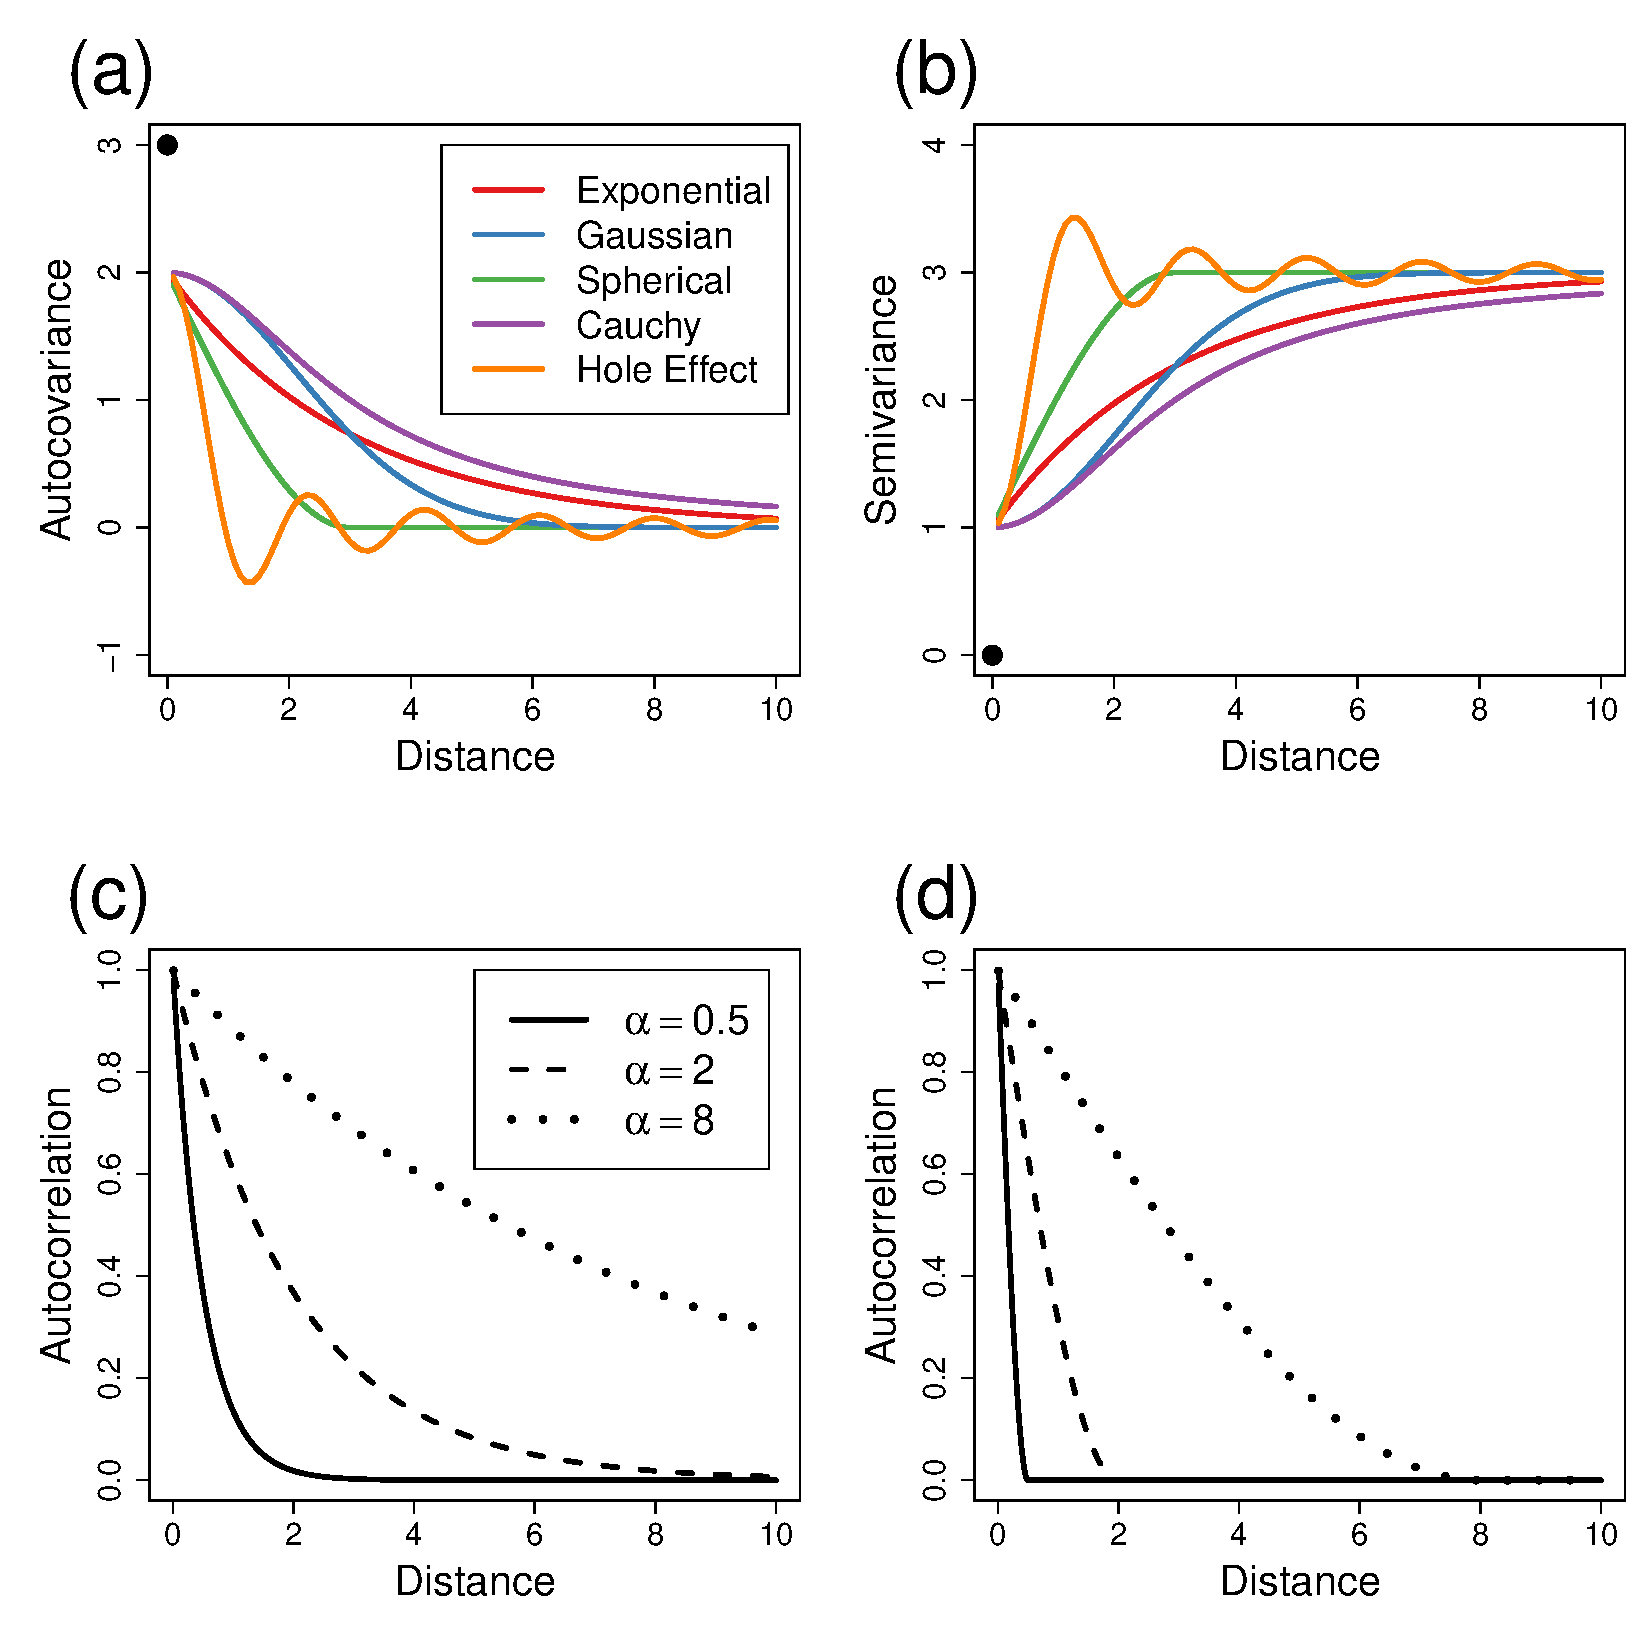
\includegraphics[width=\linewidth]{figure/Fig-autocorrModels-1.pdf}
	  \end{center}
	  \caption{Autocorrelation models. (a) Autocovariance functions for various models, with a partial sill of 2 and a nugget effect of 1. (b) The same models as in (a), except represented as semivariogram models. Effect of the range parameter $\alpha$ on the (c) exponential model, and (d) spherical model. Note that the black dots indicate a discontinuity of the fitted model at the origin due to the nugget effect, where the model ``jumps'' to the black dots when distance is exactly 0. \label{fig:autocorrModels}}
  \end{figure}


%------------------------------------------------------------------------------
%                   CautionEx
%------------------------------------------------------------------------------


	\begin{figure}[H]
	  \begin{center}
	    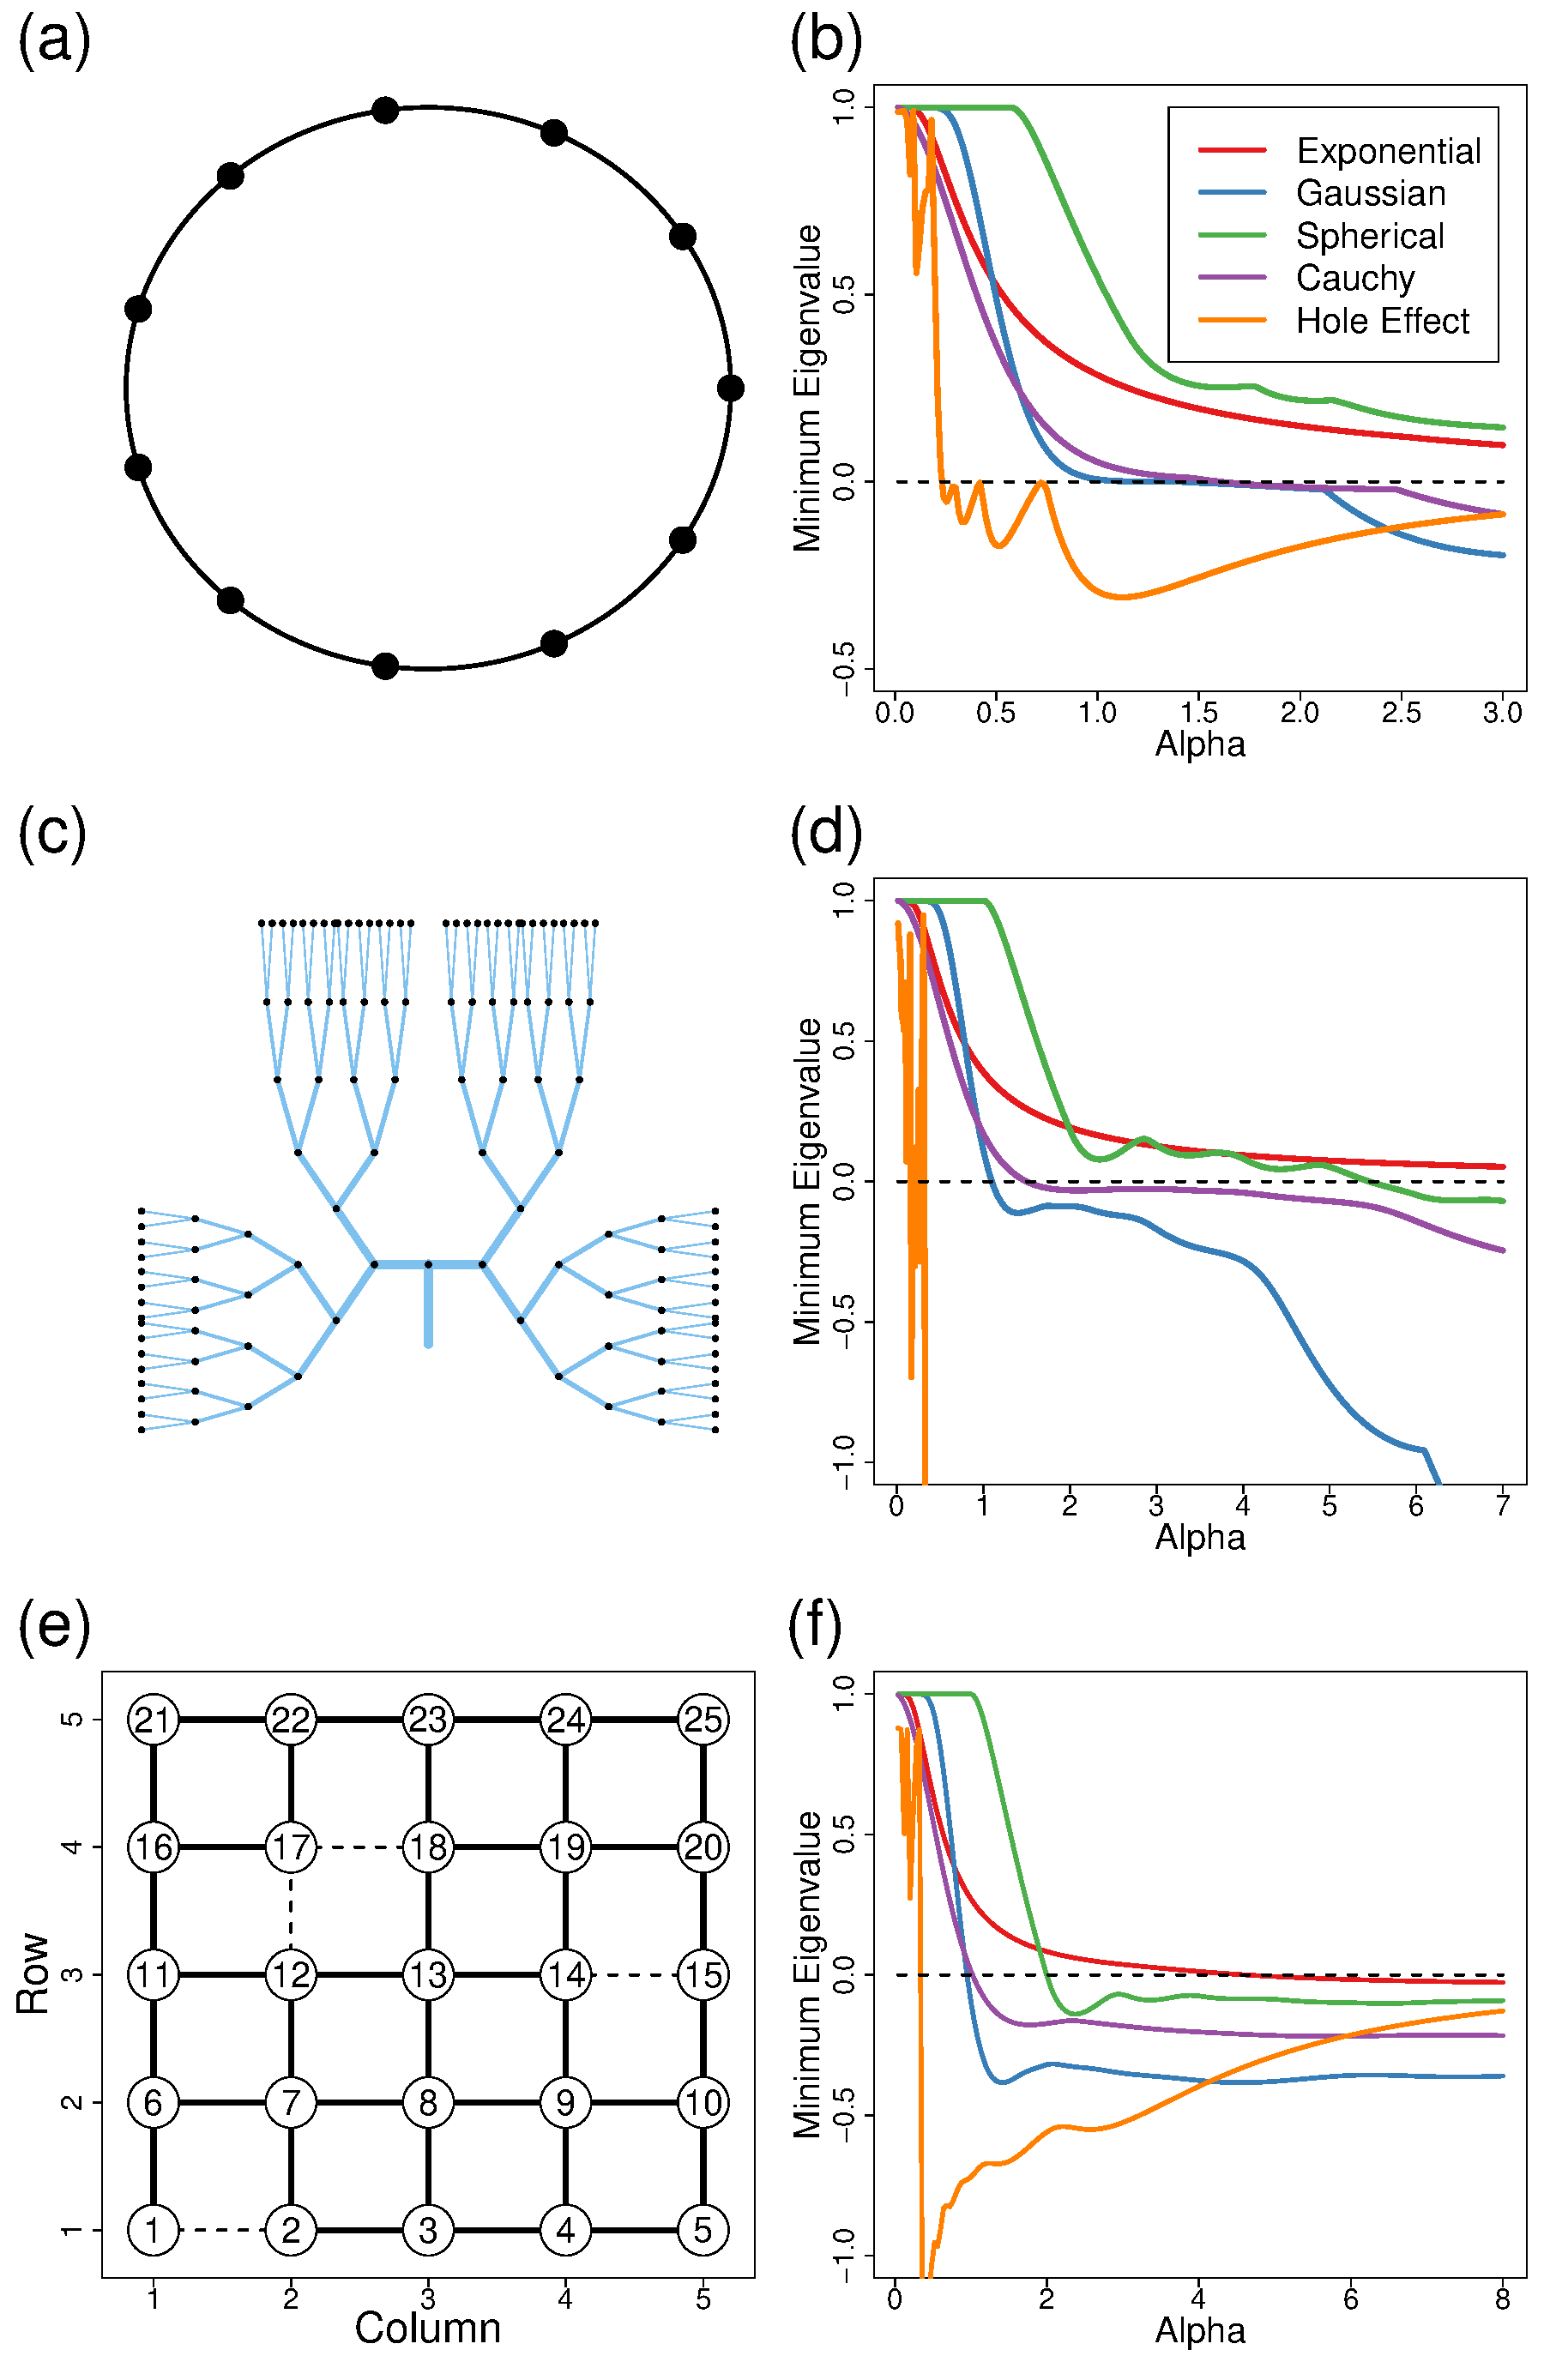
\includegraphics[width=.7\linewidth]{figure/Fig-CautionEx-1.pdf}
	  \end{center}
	  \caption{Cautionary examples. (a) 11 spatial locations on a circle are shown with solid circles. (b) Minimum eigenvalue for various autocorrelation models using distances on the circle. (c) A dichotomous branching network (stream) with 127 spatial locations at the node of each branch. (d) Minimum eigenvalue for various autocorrelation models using in-stream distance only. (e) 25 spatial locations on a grid network, where a perfect lattice includes the dashed line, but an irregular lattice includes only the solid lines. (f) Minimum eigenvalue for various autocorrelation models using shortest path distances along the irregular lattice. \label{fig:cautionEx}}
  \end{figure}

%------------------------------------------------------------------------------
%                   realLinDistEigVals
%------------------------------------------------------------------------------


	\begin{figure}[H]
	  \begin{center}
	    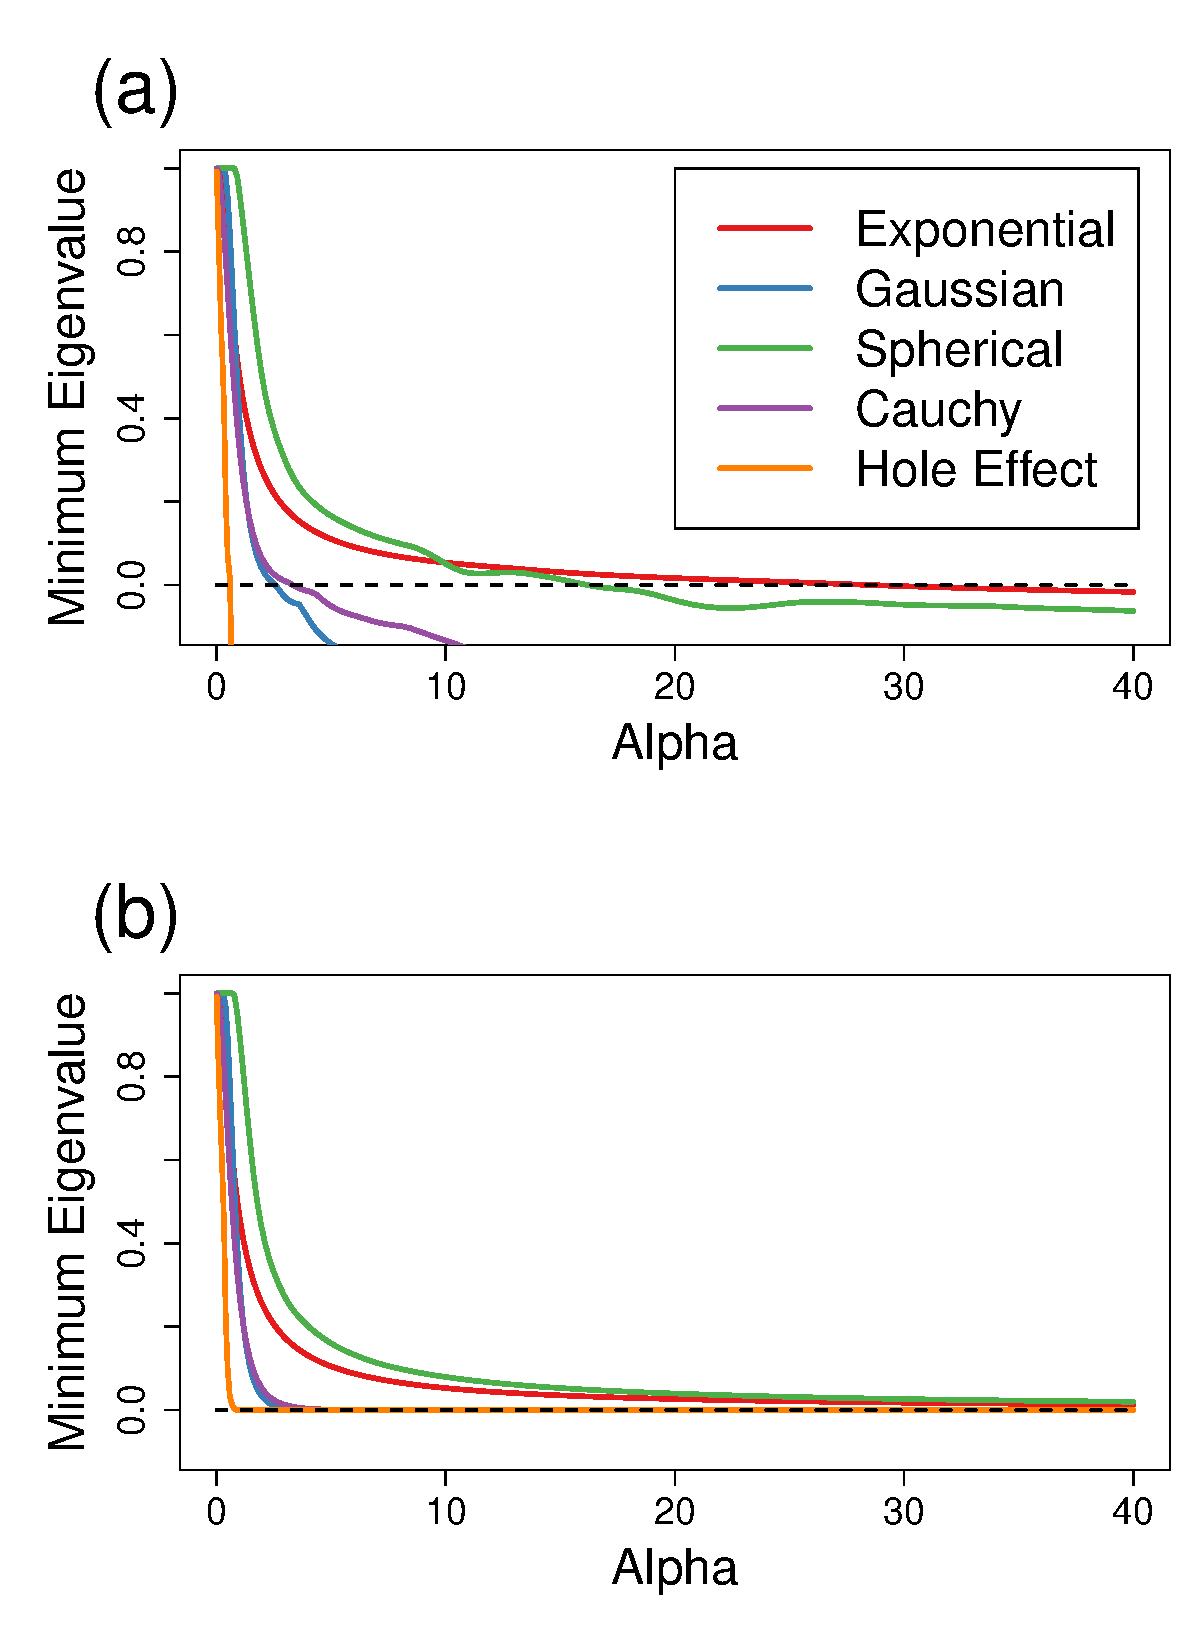
\includegraphics[width=.7\linewidth]{figure/Fig-realDatEigVals-1.pdf}
	  \end{center}
	  \caption{Minimum eigenvalues for various autocorrelation models for Ladle et al. (2016) data set. (a) Using linear distances among cameras. (b) Using Euclidean distances among cameras.  \label{fig:realLinDistEigVals}}
  \end{figure}

%------------------------------------------------------------------------------
%                   reduRank
%------------------------------------------------------------------------------


	\begin{figure}
	  \centering
      \begin{subfigure}[b]{0.5\textwidth}
      \centering
      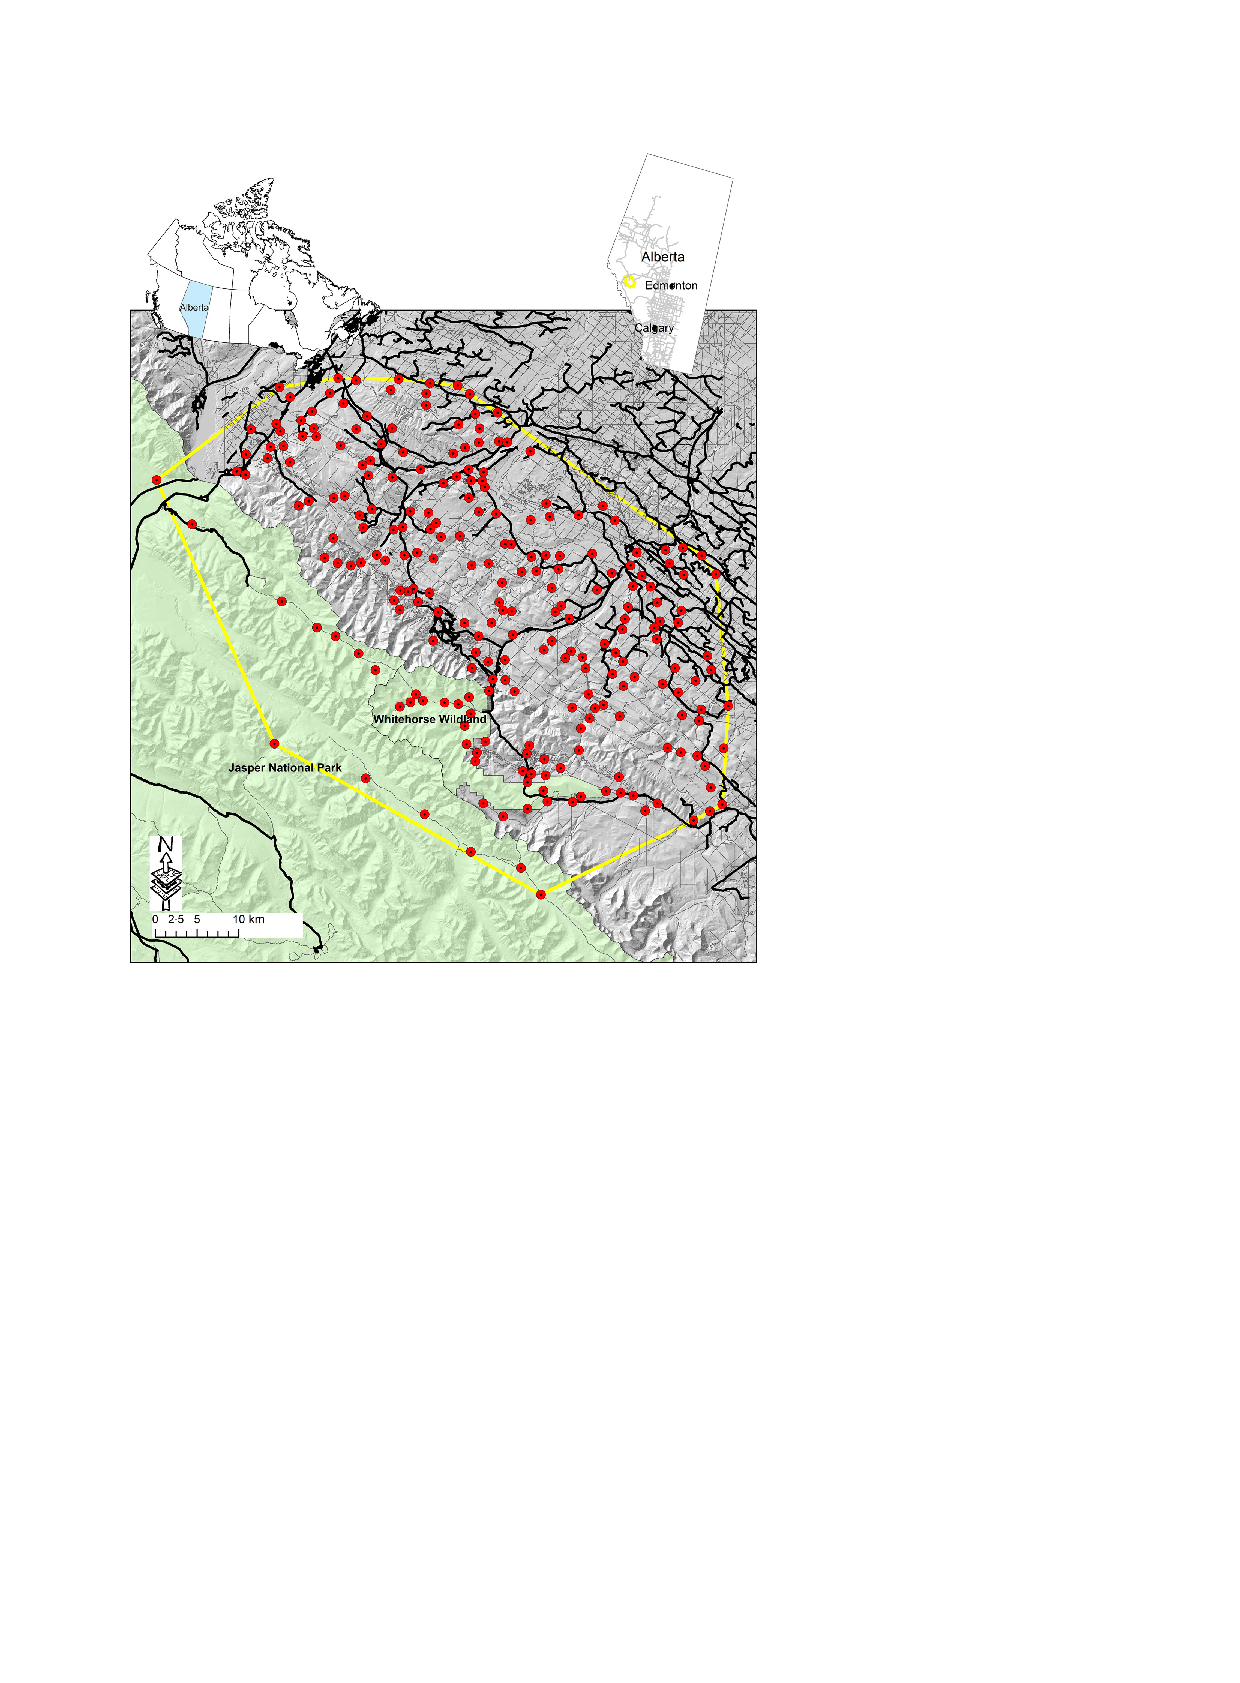
\includegraphics[width=\linewidth]{figure/Fig-LadleStudyArea-1.pdf}
      \caption{}
      \end{subfigure}%
      \begin{subfigure}[b]{0.5\textwidth}
      \centering
	    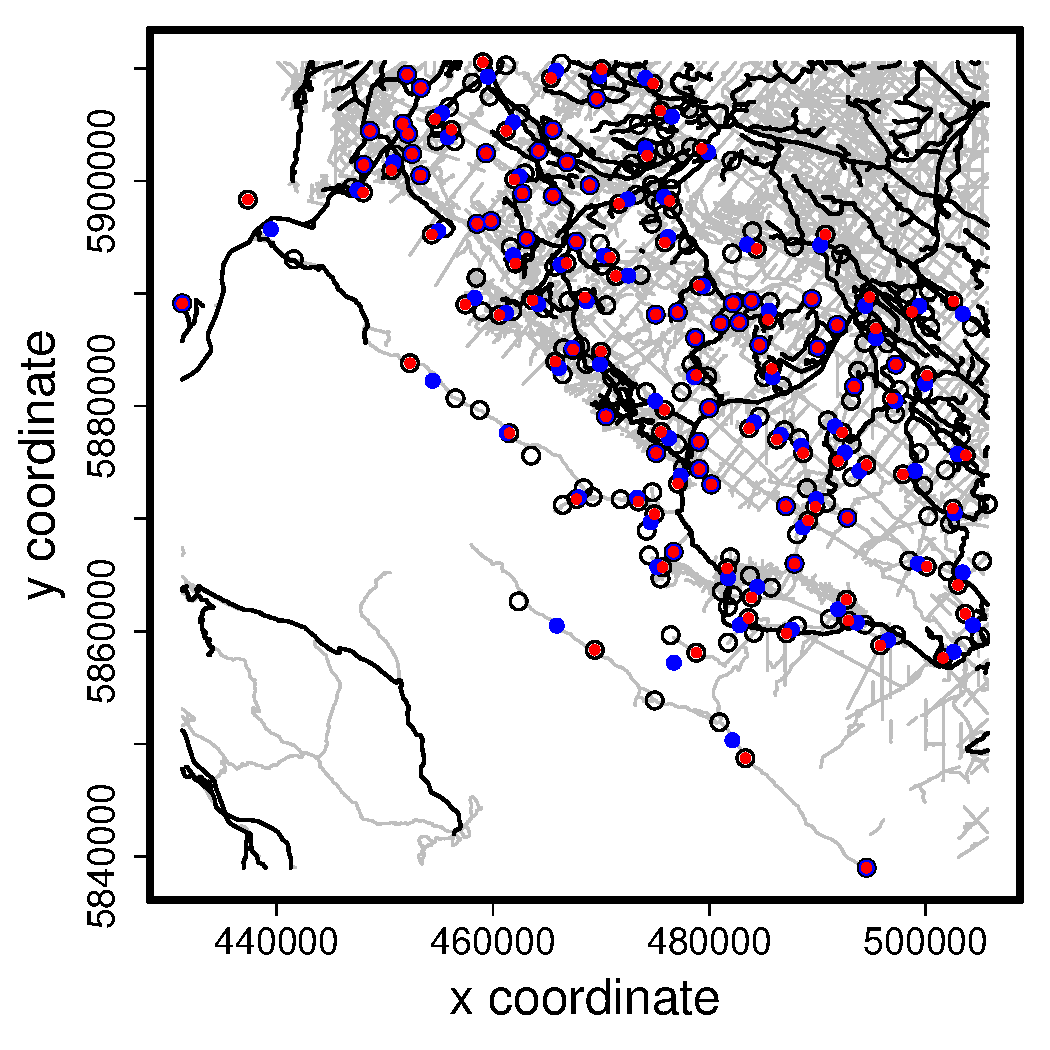
\includegraphics[width=\linewidth]{figure/Fig-knotLocs-1.pdf}
      \caption{}
      \end{subfigure}
	  \caption{(a) Study area, [will seek permission to reprint], from Ladle et al. (2017). Roads are shown as black lines, trails as gray lines, and camera locations as solid red circles. (b) All spatial locations (open circles) and knot locations for reduced-rank methods.  Initially, k-means on x- and y-coordinates created 120 clusters with center locations given by solid blue circles, and then these were moved to nearest actual locations (solid red circles).  Note that there is some discrepancy between the map in Ladle et al. (2017), (a), and the on-line data, (b), especially along the western and southern borders.  All analyses in this paper used the on-line data.}\label{fig:reduRank}
  \end{figure}

%------------------------------------------------------------------------------
%                   empSemivar
%------------------------------------------------------------------------------


	\begin{figure}[H]
	  \begin{center}
	    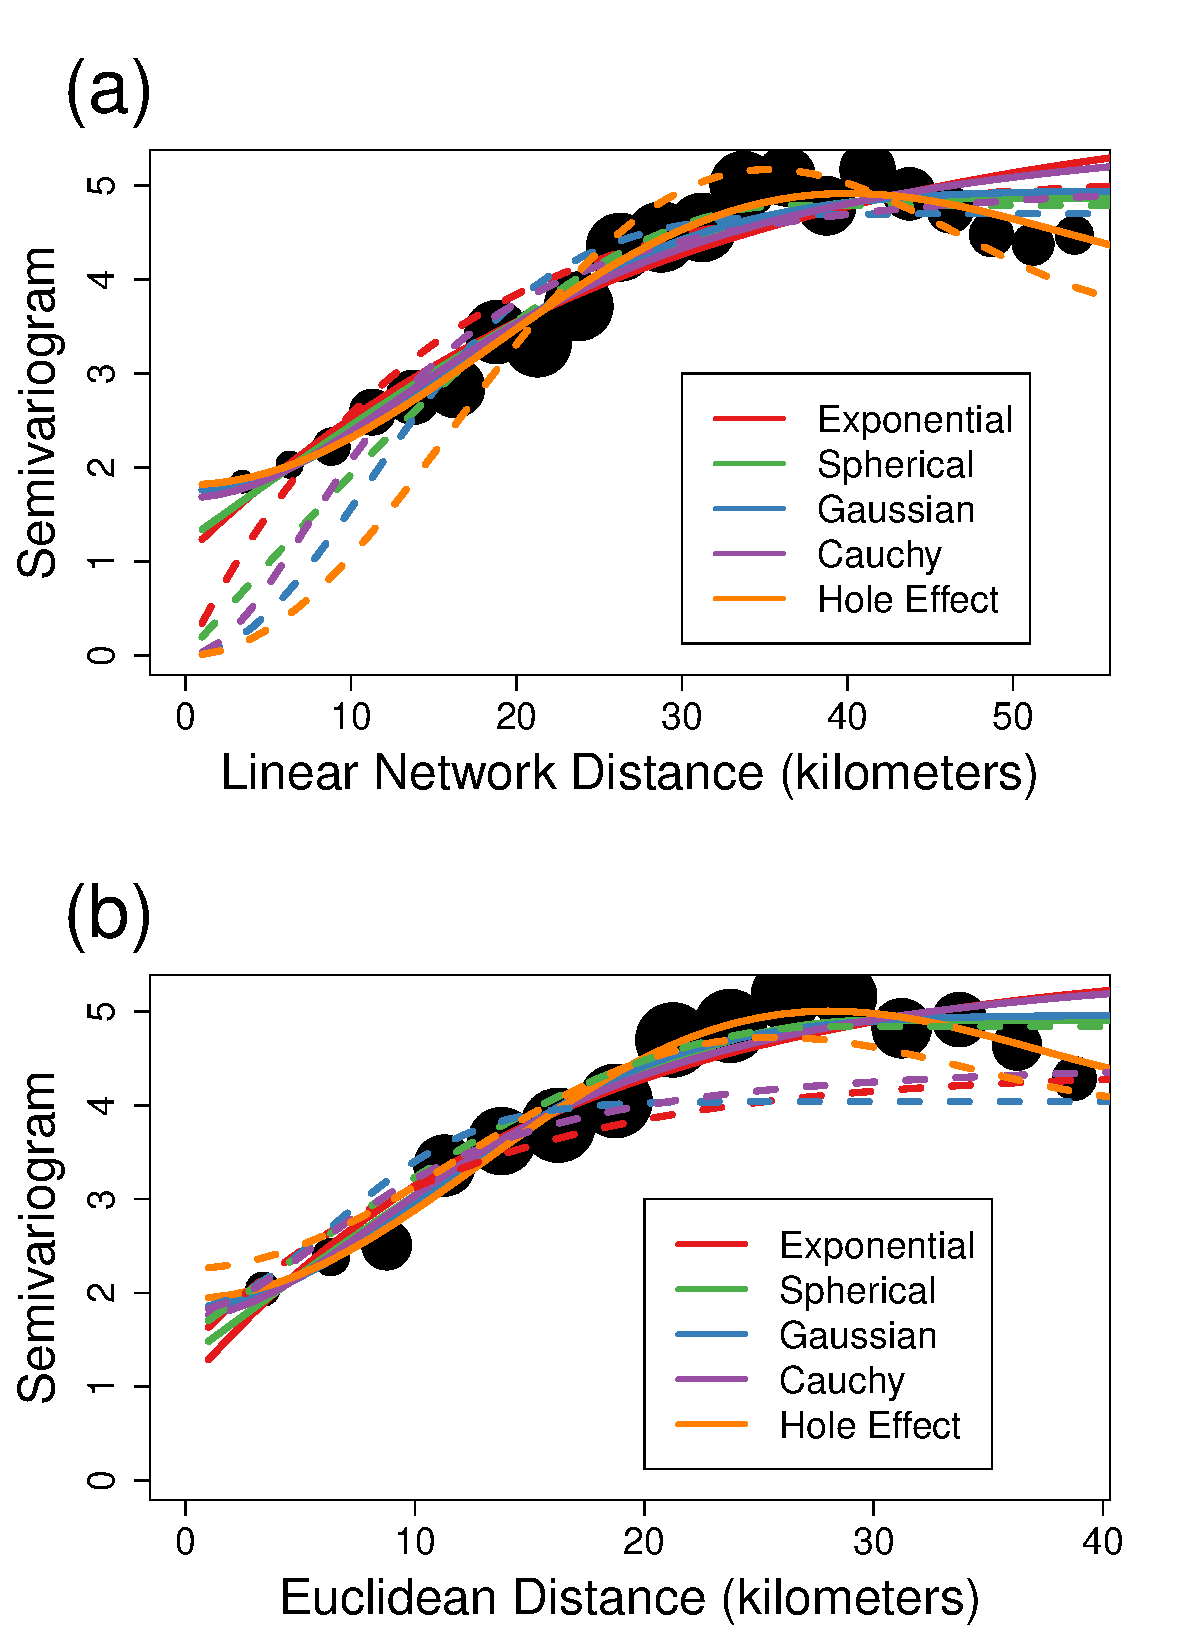
\includegraphics[width=.8\linewidth]{figure/Fig-empSemivar-1.pdf}
	  \end{center}
	  \caption{Empirical semivariogram with various fits. The solid black circles are empirical semivariogram values in distance classes, with size proportional to number of pairs of points in each distance class. (a) Linear network distances, where the dashed lines are fitted models without a nugget effect using WLS, and the solid lines are fitted models with a nugget effect using CWLS. (b) Euclidean distances, where the solid lines use CWLS, and the dashed lines use REML (which are not actually fit to the empirical semivariograms) \label{fig:empsvgm}}
  \end{figure}

%------------------------------------------------------------------------------
%                   EucLinScatter
%------------------------------------------------------------------------------


	\begin{figure}[H]
	  \begin{center}
	    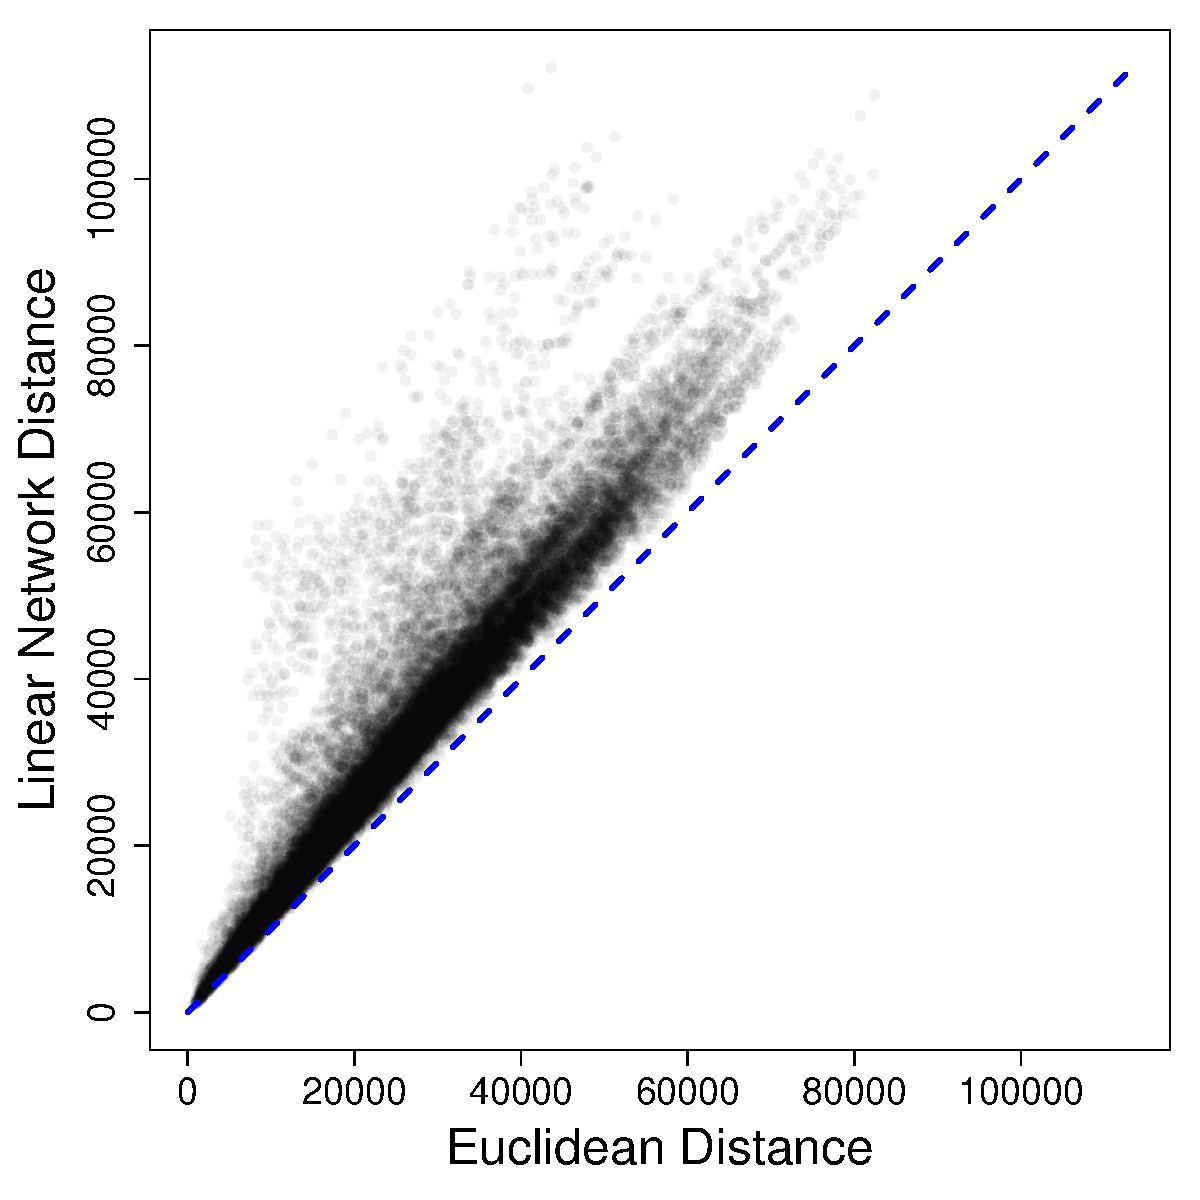
\includegraphics[width=.7\linewidth]{figure/Fig-EucLinScatter-1.pdf}
	  \end{center}
	  \caption{Scatter plot of Euclidean distance versus linear network distance for real data example.  The points are semitransparent to reveal a strong correlation between distance metrics.   \label{fig:EucLinScatter}}
  \end{figure}


\end{singlespace}
\end{flushleft}

%%%%%%%%%%%%%%%%%%%%%%%%%%%%%%%%%%%%%%%%%%%%%%%%%%%%%%%%%%%%%%%%%%%%%%%%%%%%%%%%%%
%%%%%%%%%%%%%%%%%%%%%%%%%%%%%%%%%%%%%%%%%%%%%%%%%%%%%%%%%%%%%%%%%%%%%%%%%%%%%%%%%%
%              Supplemental Material S1
%%%%%%%%%%%%%%%%%%%%%%%%%%%%%%%%%%%%%%%%%%%%%%%%%%%%%%%%%%%%%%%%%%%%%%%%%%%%%%%%%%
%%%%%%%%%%%%%%%%%%%%%%%%%%%%%%%%%%%%%%%%%%%%%%%%%%%%%%%%%%%%%%%%%%%%%%%%%%%%%%%%%%

%------------------------------------------------------------------------------
%          Supplemental Material S1: Estimation Methods
%------------------------------------------------------------------------------

\clearpage
\setcounter{equation}{0}
\renewcommand{\theequation}{eqn S.\arabic{equation}}
\setcounter{figure}{0}
\renewcommand{\thefigure}{S\arabic{figure}}
\section*{SUPPLEMENTAL MATERIAL}

\subsection*{Estimation Methods}
I use two methods to fit theoretical semivariograms \ref{eq:autocorrModels} to empirical semivariograms \ref{eq:gammahat}.  The first is simple weighted least squares.  To show the dependence of the theoretical semivariogram on parameters, write any of the models, \ref{eq:autocorrModels}, in semivariogram form with a nugget effect, $\gamma(h_k|\btheta) = \sigma^2_0 + \sigma^2_p(1 - \rho_m(h_k|\alpha))$, where $\btheta = (\sigma^2_p, \sigma^2_0, \alpha)$.  Then the weighted least squares estimator of $\btheta$ is,
\[
\hat{\btheta}_{WLS} = \argmin_{\btheta} \sum_{k=1}^K [N(\cD_k)](\hat{\gamma}(h_k) - \gamma(h_k|\btheta))^2.
\]
Cressie's weighted least squares estimate of $\btheta$ is,
\[
\hat{\btheta}_{CWLS} = \argmin_{\btheta} \sum_{k=1}^K [N(\cD_k)]\left(\frac{\hat{\gamma}(h_k)}{\gamma(h_k|\btheta)} - 1\right)^2.
\]
REML does not use an empirical semivariogram.  Rather, let $\by$ be a vector of observed data of length $n$, $\bX$ a fixed effects design matrix with $n$ rows and $p$ linearly independent columns, $\bSigma_{\btheta}$ an $n \times n$ covariance matrix, in the same order as the data, that depends on distances between observations, and a set of parameters, as given in \ref{eq:bSigma}.  Note that I show the dependence of $\bSigma$ on $\btheta$ with a subscript. Then REML estimates are given by
\begin{equation} \label{eq:REML}
	\begin{array}{c}
					\hat{\btheta}_{REML}  = \underset{\btheta}{\mathrm{argmin}} \hspace{.1cm} [(\bm Y - \bX\bbeta_g)\upp\bSigma_{\btheta}\upi(\bm Y - \bX\bbeta_g) + \log(|\bSigma_{\btheta}|) + \\
					\log(|\bX\upp\bSigma_{\btheta}\upi\bX|) + (n-p)\log(2\pi)],
	\end{array}
\end{equation}
where 
\begin{equation}\label{eq:betaHat}
				\bbeta_g = (\bX\upp\bSigma_{\btheta}\upi\bX)\upi\bX\upp\bSigma_{\btheta}\upi\bm Y
\end{equation}
is the generalized least squares estimator of $\bbeta$. Note that for our case, $\bX = \bone$, where $\bone$ is a vector of all 1s, and $\bbeta = \mu$, a scalar.

\subsection*{Simple Example on Negative Variances from Improper Covariance Matrices}

For a very simple, worked example in \texttt{R} on how a covariance matrix that is not positive definite can lead to negative variances, consider the 4 locations in a linear network shown in Figure~\ref{fig:App4LocNet}.
%%%%%%%%%%%%%%%%%%%%%%%%%%%%%%%%%%%%%%%%%%%%%%%%%%%%%%%%%%%%%%%%%%%%%%%%%%%%%%%%
%%%%%%%%%%%%%%%%%%%%%%%%%%%%%%%%%%%%%%%%%%%%%%%%%%%%%%%%%%%%%%%%%%%%%%%%%%%%%%%%
%   Simple 4 location network
%%%%%%%%%%%%%%%%%%%%%%%%%%%%%%%%%%%%%%%%%%%%%%%%%%%%%%%%%%%%%%%%%%%%%%%%%%%%%%%%
%%%%%%%%%%%%%%%%%%%%%%%%%%%%%%%%%%%%%%%%%%%%%%%%%%%%%%%%%%%%%%%%%%%%%%%%%%%%%%%%

	\begin{figure}[H]
	  \begin{center}
	    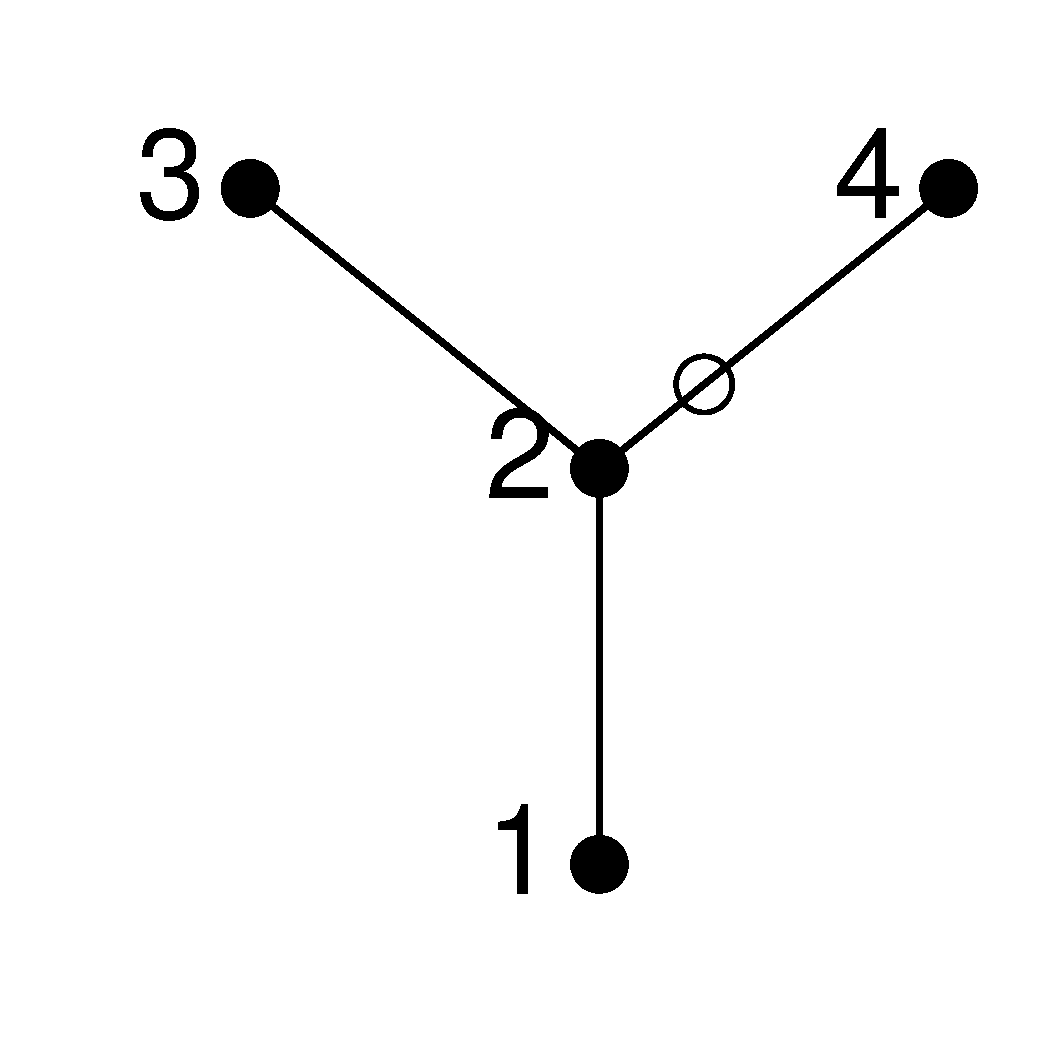
\includegraphics[width=.3\linewidth]{figure/Fig-App4LocNetwork-1.pdf}
	  \end{center}
	  \caption{A simple 4-location network, where each location is given by a solid circle numbered from 1 to 4, along with a prediction location, shown by the open circle. \label{fig:App4LocNet}}
  \end{figure}
\noindent
Let the linear distance between each connected location be 1 unit, so the distance matrix among the 4 locations, numbered sequentially for the rows and columns, is
\begin{singlespace}
\begin{knitrout}
\definecolor{shadecolor}{rgb}{0.969, 0.969, 0.969}\color{fgcolor}\begin{kframe}
\begin{alltt}
\hlstd{linDmat} \hlkwb{=} \hlkwd{rbind}\hlstd{(}
  \hlkwd{c}\hlstd{(}\hlnum{0}\hlstd{,}\hlnum{1}\hlstd{,}\hlnum{2}\hlstd{,}\hlnum{2}\hlstd{),}
  \hlkwd{c}\hlstd{(}\hlnum{1}\hlstd{,}\hlnum{0}\hlstd{,}\hlnum{1}\hlstd{,}\hlnum{1}\hlstd{),}
  \hlkwd{c}\hlstd{(}\hlnum{2}\hlstd{,}\hlnum{1}\hlstd{,}\hlnum{0}\hlstd{,}\hlnum{2}\hlstd{),}
  \hlkwd{c}\hlstd{(}\hlnum{2}\hlstd{,}\hlnum{1}\hlstd{,}\hlnum{2}\hlstd{,}\hlnum{0}\hlstd{))}
\end{alltt}
\end{kframe}
\end{knitrout}
\[
\bD = \left(
\begin{array}{cccc}
% latex table generated in R 3.4.1 by xtable 1.8-2 package
% Sun Nov 12 16:36:40 2017
 0 & 1 & 2 & 2 \\ 
  1 & 0 & 1 & 1 \\ 
  2 & 1 & 0 & 2 \\ 
  2 & 1 & 2 & 0 \\ 
  
\end{array}
\right)
\]
\end{singlespace}
\noindent I will use the Gaussian autocorrelation model, \ref{eq:autocorrModels}, with $\sigma^2_p = 1$, $\alpha = 3$, and a small nugget effect, $\sigma_0 = 0.01$.  
\begin{knitrout}
\definecolor{shadecolor}{rgb}{0.969, 0.969, 0.969}\color{fgcolor}\begin{kframe}
\begin{alltt}
\hlstd{Sig} \hlkwb{=} \hlkwd{exp}\hlstd{(}\hlopt{-}\hlstd{(linDmat}\hlopt{/}\hlnum{3}\hlstd{)}\hlopt{^}\hlnum{2}\hlstd{)} \hlopt{+} \hlkwd{diag}\hlstd{(}\hlkwd{rep}\hlstd{(}\hlnum{0.01}\hlstd{,} \hlkwc{times} \hlstd{=} \hlnum{4}\hlstd{))}
\end{alltt}
\end{kframe}
\end{knitrout}
\begin{singlespace}
\begin{equation} \label{eq:appSigma}
\bSigma = \left(
\begin{array}{cccc}
% latex table generated in R 3.4.1 by xtable 1.8-2 package
% Sun Nov 12 16:36:40 2017
 1.010 & 0.895 & 0.641 & 0.641 \\ 
  0.895 & 1.010 & 0.895 & 0.895 \\ 
  0.641 & 0.895 & 1.010 & 0.641 \\ 
  0.641 & 0.895 & 0.641 & 1.010 \\ 
  
\end{array}
\right)
\end{equation}
\end{singlespace}
\noindent The spectral decomposition, $\bSigma = \bQ\bLambda\bQ\upp$ (\ref{eq:spectralDecomp}) is
\begin{singlespace}
\begin{knitrout}
\definecolor{shadecolor}{rgb}{0.969, 0.969, 0.969}\color{fgcolor}\begin{kframe}
\begin{alltt}
\hlstd{Lambda} \hlkwb{=} \hlkwd{diag}\hlstd{(}\hlkwd{eigen}\hlstd{(Sig)}\hlopt{$}\hlstd{values)}
\hlstd{Q} \hlkwb{=} \hlkwd{eigen}\hlstd{(Sig)}\hlopt{$}\hlstd{vectors}
\end{alltt}
\end{kframe}
\end{knitrout}
\begin{equation} \label{eq:appSpecDeco}
\bLambda= \left(
\begin{array}{cccc}
% latex table generated in R 3.4.1 by xtable 1.8-2 package
% Sun Nov 12 16:36:40 2017
 3.328 & 0.000 & 0.000 & 0.000 \\ 
  0.000 & 0.369 & 0.000 & 0.000 \\ 
  0.000 & 0.000 & 0.369 & 0.000 \\ 
  0.000 & 0.000 & 0.000 & -0.026 \\ 
  
\end{array}
\right)
\hspace{.3cm}
\bQ = \left(
\begin{array}{cccc}
% latex table generated in R 3.4.1 by xtable 1.8-2 package
% Sun Nov 12 16:36:40 2017
 -0.480 & 0.000 & 0.816 & -0.321 \\ 
  -0.556 & -0.000 & 0.000 & 0.831 \\ 
  -0.480 & -0.707 & -0.408 & -0.321 \\ 
  -0.480 & 0.707 & -0.408 & -0.321 \\ 
  
\end{array}
\right)
\end{equation}
\end{singlespace}
\noindent The eigenvectors, $\bv_i; i = 1,\ldots,4$, in $\bQ = [\bv_1|\bv_2|\bv_3|\bv_4]$ are orthonormal, which means that $\bv_i\upp \bv_j = 0$ if $i \ne j$, but $\bv_i\upp \bv_i = 1$.
\begin{singlespace}
\begin{knitrout}
\definecolor{shadecolor}{rgb}{0.969, 0.969, 0.969}\color{fgcolor}\begin{kframe}
\begin{alltt}
\hlstd{Q[,}\hlnum{1}\hlstd{]} \hlopt \hlstd{Q[,}\hlnum{4}\hlstd{]}
\end{alltt}
\begin{verbatim}
##              [,1]
## [1,] 2.775558e-17
\end{verbatim}
\begin{alltt}
\hlstd{Q[,}\hlnum{4}\hlstd{]} \hlopt \hlstd{Q[,}\hlnum{4}\hlstd{]}
\end{alltt}
\begin{verbatim}
##      [,1]
## [1,]    1
\end{verbatim}
\end{kframe}
\end{knitrout}
\end{singlespace}

Now, consider 4 random variables, $\bm Y = \{Y_1,Y_2,Y_3,Y_4\}$. The linear combination $\bv_4\upp\bm Y = -0.321Y_1 + 0.831Y_2 - 0.321Y_3 - 0.321Y_4$ is a perfectly valid construction, and must have a positive variance.  However, if $\bm Y$ has covariance matrix $\bSigma$ in \ref{eq:appSigma}, then $\var(\bv_4\upp\bm Y) = \bv_4\upp\bSigma\bv_4 = -0.026$, which is the 4th eigenvalue,
\begin{singlespace}
\begin{knitrout}
\definecolor{shadecolor}{rgb}{0.969, 0.969, 0.969}\color{fgcolor}\begin{kframe}
\begin{alltt}
\hlstd{v4} \hlkwb{=} \hlstd{Q[,}\hlnum{4}\hlstd{]}
\hlkwd{t}\hlstd{(v4)} \hlopt \hlstd{Sig} \hlopt \hlstd{v4}
\end{alltt}
\begin{verbatim}
##             [,1]
## [1,] -0.02611639
\end{verbatim}
\end{kframe}
\end{knitrout}
\end{singlespace}
\noindent which is not a valid variance, so $\bSigma$ in \ref{eq:appSigma} is not a valid covariance matrix.

To show how this works for kriging, consider predicting the location shown with the open circle in Figure~\ref{fig:App4LocNet}, which is 3/10 of the way from location 2 to location 4.  Then the distance from the 4 locations with solid circles in Figure~\ref{fig:App4LocNet} to the prediction location is the vector $(1.3, 0.3, 1.3, 0.7)$, and the covariances between the prediction location and the 4 locations with solid circles in Figure~\ref{fig:App4LocNet} is 
\begin{singlespace}
\begin{knitrout}
\definecolor{shadecolor}{rgb}{0.969, 0.969, 0.969}\color{fgcolor}\begin{kframe}
\begin{alltt}
\hlstd{cvec} \hlkwb{=} \hlkwd{exp}\hlstd{(}\hlopt{-}\hlstd{(}\hlkwd{c}\hlstd{(}\hlnum{1.3}\hlstd{,} \hlnum{0.3}\hlstd{,} \hlnum{1.3}\hlstd{,} \hlnum{0.7}\hlstd{)}\hlopt{/}\hlnum{3}\hlstd{)}\hlopt{^}\hlnum{2}\hlstd{)}
\hlstd{cvec}
\end{alltt}
\begin{verbatim}
## [1] 0.8287989 0.9900498 0.8287989 0.9470111
\end{verbatim}
\end{kframe}
\end{knitrout}
\end{singlespace}
\noindent Using \ref{eq:OKse}, the prediction variance of the location with the open circle, using data from the locations with the solid black circles, would be computed as
\begin{singlespace}
\begin{knitrout}
\definecolor{shadecolor}{rgb}{0.969, 0.969, 0.969}\color{fgcolor}\begin{kframe}
\begin{alltt}
\hlstd{(}\hlnum{1} \hlopt{+} \hlnum{0.01}\hlstd{)} \hlopt{-} \hlkwd{t}\hlstd{(cvec)} \hlopt \hlkwd{solve}\hlstd{(Sig)} \hlopt \hlstd{cvec} \hlopt{+}
  \hlstd{(}\hlnum{1} \hlopt{-} \hlstd{(}\hlkwd{sum}\hlstd{(}\hlkwd{solve}\hlstd{(Sig)} \hlopt \hlstd{cvec))}\hlopt{^}\hlnum{2}\hlstd{)}\hlopt{/}\hlkwd{sum}\hlstd{(}\hlkwd{solve}\hlstd{(Sig))}
\end{alltt}
\begin{verbatim}
##            [,1]
## [1,] -0.0425027
\end{verbatim}
\end{kframe}
\end{knitrout}
\end{singlespace}
\noindent which is negative, so we see that the larger matrix, where $\bSigma$ is appended with covariances that include the prediction location, \ref{eq:ObPredSig}, is not a valid covariance matrix. 


%%%%%%%%%%%%%%%%%%%%%%%%%%%%%%%%%%%%%%%%%%%%%%%%%%%%%%%%%%%%%%%%%%%%%%%%%%%%%%%%%%
%%%%%%%%%%%%%%%%%%%%%%%%%%%%%%%%%%%%%%%%%%%%%%%%%%%%%%%%%%%%%%%%%%%%%%%%%%%%%%%%%%
%%%%%%%%%%%            %%%%%%%    %%%%%%%%  %%%%%%%       %%%%%%%%%%%%%%%%%%%%%%%%
%%%%%%%%%%%  %%%%%%%%%%%%%%%%%  %  %%%%%%%  %%%%%%%  %%%%  %%%%%%%%%%%%%%%%%%%%%%%
%%%%%%%%%%%  %%%%%%%%%%%%%%%%%  %%  %%%%%%  %%%%%%%  %%%%%%  %%%%%%%%%%%%%%%%%%%%%
%%%%%%%%%%%  %%%%%%%%%%%%%%%%%  %%%  %%%%%  %%%%%%%  %%%%%%%   %%%%%%%%%%%%%%%%%%%
%%%%%%%%%%%            %%%%%%%  %%%%  %%%%  %%%%%%%  %%%%%%%%  %%%%%%%%%%%%%%%%%%%
%%%%%%%%%%%  %%%%%%%%%%%%%%%%%  %%%%%  %%%  %%%%%%%  %%%%%%%   %%%%%%%%%%%%%%%%%%%
%%%%%%%%%%%  %%%%%%%%%%%%%%%%%  %%%%%%  %%  %%%%%%%  %%%%%%  %%%%%%%%%%%%%%%%%%%%%
%%%%%%%%%%%  %%%%%%%%%%%%%%%%%  %%%%%%%  %  %%%%%%%  %%%%  %%%%%%%%%%%%%%%%%%%%%%%
%%%%%%%%%%%            %%%%%%%  %%%%%%%%    %%%%%%%       %%%%%%%%%%%%%%%%%%%%%%%%
%%%%%%%%%%%%%%%%%%%%%%%%%%%%%%%%%%%%%%%%%%%%%%%%%%%%%%%%%%%%%%%%%%%%%%%%%%%%%%%%%%
%%%%%%%%%%%%%%%%%%%%%%%%%%%%%%%%%%%%%%%%%%%%%%%%%%%%%%%%%%%%%%%%%%%%%%%%%%%%%%%%%%


\end{spacing}

\end{document}


